\documentclass[green, fancy, 11pt]{elegantbook}

\usepackage{lscape}
\usepackage{float}
\usepackage[italian]{babel}

\definecolor{RussianGreen}{RGB}{102, 150, 111}
\definecolor{OldLace}{RGB}{248, 250, 229}
\definecolor{Asparagus}{RGB}{135, 169, 107}
\definecolor{BudGreen}{RGB}{123, 182, 97}
\definecolor{Green}{RGB}{0, 128, 0}
\definecolor{DarkGreen}{RGB}{27,108,68}

\definecolor{customcolor}{RGB}{27,108,68}
\colorlet{coverlinecolor}{customcolor}

\title{Progettazione Software AnconAmbiente}
\subtitle{Esame Ingegneria del Software}

\author{Lorenzo Benenchia, Lorenzo Cardoni, Rahmi El Mechri, Riccardo Iobbi}
\institute{UNIVPM}
\date{May. 4, 2021}
\logo{UNIVPM_logo.png}
\cover{cover2.png}

\begin{document}

\maketitle
\frontmatter
\tableofcontents
\mainmatter

\chapter{INTRODUZIONE}
AnconAmbiente Spa è il maggiore gestore dei servizi di igiene urbana della provincia di Ancona.
E’ nel comune di Ancona che l’Azienda gestisce numericamente più servizi, infatti oltre all’igiene urbana (raccolta rifiuti solidi urbani e differenziati, pulizia e spazzamento), che rappresenta il principale settore, Anconambiente gestisce i servizi di pubblica illuminazione (riqualificazione e manutenzione), servizi cimiteriali e lampade votive. In passato si è anche occupata della gestione dei servizi di ventilazione gallerie, 
pubbliche affissioni e prevenzione infestanti.
Uno schema dell'organizzazione dell'area tecnica operativa è visibile in figura \ref{organigramma}:

\begin{figure}[H]
	\centering
	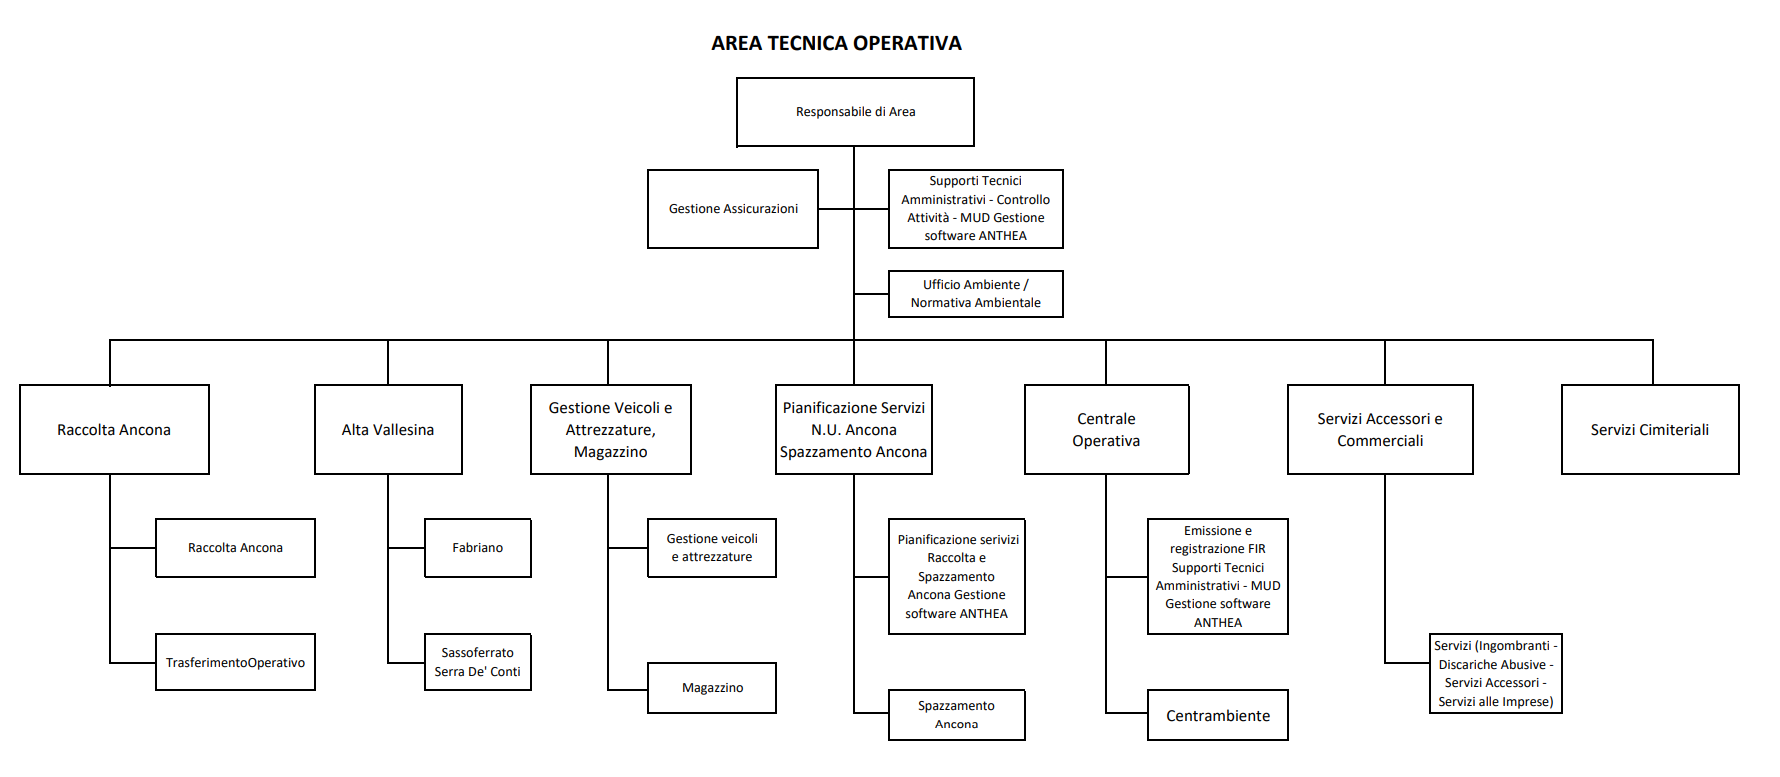
\includegraphics[width=15cm,scale=0.5]{schema_AA}\\
	\caption{Organizzazione area tecnica operativa}
	\label{organigramma}
\end{figure}
\newpage

\section{Intervista}
A Maggio 2021 è stata effettuata una intervista a distanza (a causa pandemia) con il Sir. Andrea Cardoni.
Questa intervista ha come scopo di capire come funziona l'aziende e come vengono gestite le varie attività.
A seguire viene riportata la trascrizione parziale dell'intervista contenente le parti fondamentali per la progettazione del software.

\begin{itemize}
	\item \textbf{Qual è lo scopo del programma?}\\
	Il programma deve aiutare a gestire i servizi e la programmazione dei clienti.
	
	\item \textbf{Avete già un programma che se ne occupa?}\\
	Si, al momento stiamo utilizzando un programma che si chiama Anthea, un ERP specifico per il settore ambientale, quindi utilizzato da aziende come la nostra.
	
	\item \textbf{Chi utilizza il programma?}\\
	Il programma viene utilizzato da utenti con responsabilità diverse. I responsabili d'area si occupano
	della visualizzazione dei report, il responsabile amministrativo si occupa della parte di calcolo costi e fatturazioni. I lavoratori dell'ufficio tecnico gestiscono invece la coordinazione degli operatori e dei mezzi per il completamento dei servizi. Inoltre i dipendenti dell'officina dell'azienda si occupano della manutenzione dei mezzi.
	
	\item \textbf{Anche gli operatori hanno accesso al programma?}\\
	No, gli operatori utilizzano una app che permette loro di vedere i propri turni.
	
	\item \textbf{Quindi ogni utente ha dei privilegi diversi?}\\
	Si, il programma è diviso in moduli, ogni settore ha i propri ruoli, e possono accedere solamente a
	certi moduli a seconda delle loro responsabilità, ad eccezione dell'amministratore di sistema, e dei responsabili.
	E' proprio l'amministratore di sistema che si occupa della gestione delle credenziali e degli accessi.
	
	\item \textbf{Quali servizi offrite?}\\
	Ci occupiamo di igiene ambientale, più in particolare di raccolta rifiuti, pulizia delle aree pubbliche, smaltimento dei rifiuti, gestione dei centri di raccolta.
	
	\item \textbf{Quali sono i vostri clienti?}\\
	I nostri clienti principali sono i comuni, che compongono più del 95\% del nostro lavoro. In particolare lavoriamo
	con 5 comuni: Ancona, Fabriano, Sassoferrato, Cerreto D'Esi, Serra de' Conti. Poi una piccola parte delle richieste
	arriva da privati, ad esempio dei condomini.
	
	\item \textbf{Che informazioni salvate dei vostri clienti?}\\
	Dei comuni, dobbiamo sapere da contratto che servizi dobbiamo offrire, se la gestione della fattura è affidata a noi o meno, e la partita IVA. Per quanto riguarda i privati dobbiamo sapere anagrafica e partita IVA.
	
	\item \textbf{E come arrivano le richieste da parte dei vostri clienti?}\\
	I consigli comunali richiedono il servizio, attraverso una delibera, al cda di AnconAmbiente. Quindi viene effettuata una
	indagine conoscitiva, e una rendicontazione economica. Una volta che è stato stipulato il contratto, AnconAmbiente si occuperà
	di tutti i servizi concordati. I privati invece effettuano le richiesta vie e-mail o via telefono.
	
	\item \textbf{Qual è il processo di inserimento dei servizi?}\\
	Una volta arrivata la richiesta, viene preventivato il costo, e i dipendenti dell'ufficio turni inseriscono nel sistema le informazioni relative al servizio, ovvero: il Cliente, il Codice del servizio, il tipo di servizio, l'orario, i mezzi necessari che si utilizzeranno e gli operatori, con le specializzazioni adeguate, che se ne occuperanno. Inoltre viene specificato se il servizio necessita del formulario o meno. Se si tratta di un servizio che verrà effettuato periodicamente bisognerà anche specificare che giorni della settimana sarà effettuato.
	
	\newpage
	\item \textbf{Cos'è il formulario?}\\
	Le normative richiedono che ci sia un documento di trasporto dei rifiuti, e il formulario serve proprio a questo, e deve specificare chi è il produttore di rifiuti, che tipo di rifiuti è, chi li trasporta, e dove.
	
	\item \textbf{Quali informazioni sugli operatori sono necessarie?}\\
	Per ogni operatore dobbiamo sapere l'anagrafica, incluso il codice fiscale, il periodo di assunzione, le sue specializzazioni, e il tipo di patente che possiede. Inoltre ad ognuno di essi è affidata una Matricola identificativa.
	
	\item \textbf{Come viene gestito l'inserimento di nuovi dipendenti?}\\
	L'ufficio del personale richiede all'ufficio turni di inserirli nel sistema, dando loro le informazioni necessarie.
	
	\item \textbf{Come viene gestito invece il parco mezzi?}\\
	I mezzi sono divisi in tipologia di grandezza, tipo di patente necessaria, e funzione. Ogni mezzo ha un proprio codice.
	Il personale dell'officina si occupa della loro manutenzione, ed in caso di malfunzionamento di uno dei mezzi, notificano l'indisponibilità di un mezzo attraverso l'accesso al modulo di manutenzione. Tra le diverse informazioni salvate nel sistema è presente anche lo stato dell'iscrizione del mezzo all'albo dei trasportatori, e la prossima scadenza.
	
	\item \textbf{Come avviene il calcolo dei costi dei contratti?}\\
	Una volta stipulato il contratto viene generato il costo di servizio. Questo dipende da diversi fattori, ovvero: il costo orario del personale, che varia a seconda del numero di operatori, e il loro livello di specializzazione, il costo orario del mezzo, che comprende ammortamento, consumi e la manutenzione, e infine bisogna aggiungere anche il costo gestione, ovvero una percentuale fissa in più sul totale, che momentaneamente si attesta al 18\%, ma può variare. Inoltre, in caso il servizio venga effettuato di domenica, c'è una ulteriore maggiorazione.
	
	\item \textbf{Chi decide e chi può modificare questi costi?}\\
	I responsabili amministrativi si occupano della decisione dei singoli costi, e possono quindi modificarli in caso di variazione.
	
	\item \textbf{Che cosa si intende per report?}\\
	Con report si intende la possibilità di vedere le informazioni riguardanti uno specifico soggetto, ad esempio la visualizzazione dei turni effettuati da un operatore in un lasso di tempo, o la possibilità di vedere i servizi effettuati in una certa data. Un altro report importante è la visualizzazione del periodo totale di tempo in cui un mezzo è rimasto non disponibile.
	
	\item \textbf{Che succede se un servizio viene annullato o rimandato?}\\
	Un dipendente dell'ufficio turni si occuperà di segnalare il servizio come annullato, e, in caso fosse stato rimandato, di aggiungere il servizio nella nuova data pattuita.
	
	\item \textbf{E in caso di imprevisti?}\\
	In questo caso un dipendente dell'ufficio tecnico aggiungerà questo imprevisto nei dettagli del servizio. Sono i comuni che si occupano della fase di controllo, hanno infatti accesso al sistema GPS per controllare che il servizio sia stato eseguito.
	
	\item \textbf{Ci sono eventuali processi che vorreste automatizzare?}\\
	Il sistema deve inserire periodicamente i servizi giornalieri in automatico.
\end{itemize}
\newpage

\section{Descrizione}
Viene riportata una descrizione in linguaggio naturale dell'intervista per comprendere meglio gli obiettivi che il software deve raggiungere.
\\
Il sistema da realizzare sarà utilizzato da AnconAmbiente, azienda di raccolta rifiuti che opera nel territorio della provincia di ancona.\\
\\
Lo scopo del sistema è quello di assistere l’azienda nell’operazione di gestione dei servizi offerti e la relativa programmazione dei clienti.\\
\\
L’azienda al momento dell’intervista sta già utilizzando un sistema ERP, specializzato nel settore ambientale, chiamato Anthea.\\
Il sistema da realizzare dovrà implementare un sistema di login che permetta di gestire utenti con livelli di autorizzazione differenti.\\
\\
Il sistema sarà utilizzato da figure professionali diverse tra loro; I responsabili di area devono poter visualizzare report, i responsabili amministrativi devono poter calcolare costi ed emettere fatture.\\
\\
Appaiono inoltre altre figure professionali che utilizzeranno il programma, in particolare abbiamo i dipendenti dell’ufficio tecnico, i quali usufruiranno del sistema per coordinare gli operatori e i mezzi impegnati nei vari servizi offerti e in fine i dipendenti dell’officina aziendale che si occupano della manutenzione del parco mezzi.\\
Discorso a parte va fatto per gli operatori ambientali che non avranno accesso diretto al programma ma, invece, dovranno poter visualizzare i propri turni su un’app a parte che si interfaccia con il nostro sistema informativo.\\
Ogni figura professionale che si interfaccia con il sistema avrà quindi differente accesso ai vari moduli del programma, a seconda del ruolo ricoperto e del livello di autorizzazione a loro associato, eccezion fatta per i responsabili di ogni settore e gli amministratori che avranno accesso completo ai vari moduli del sistema; Nello specifico gli amministratori saranno gli unici a poter gestire le credenziali di accesso di ogni utente registrato.\\
\\
Il sistema si occuperà di gestire i servizi offerti da AnconAmbiente ai propri clienti; I servizi includono la raccolta dei rifiuti, la pulizia delle aree pubbliche, lo smaltimento dei rifiuti e la gestione dei centri di raccolta.
I principali clienti sono i comuni, in particolare i comuni di Ancona, Fabriano, Sassoferrato, Cerreto D’Esi e Serra de ‘Conti; Una piccola parte dei clienti è rappresentata da privati.\\
\\
Il sistema deve permettere di salvare informazioni sui clienti relative al servizio richiesto, gestione della fattura e partita IVA.\\
Per i clienti privati il sistema dovrà salvare l’anagrafica e partita IVA.\\
\\
I consigli comunali richiedono il servizio al cda di AnconAmbiente, dopo viene eseguita un’indagine conoscitiva, si presenta un preventivo e il tutto viene concordato in un contratto.\\
\\
I clienti privati possono effettuare le richieste di servizio via e-mail o per chiamata telefonica.\\
\\
Per l’inserimento di un servizio nel sistema i dipendenti dell’ufficio turni inseriranno le informazioni necessarie che includono il cliente, il codice del servizio, il tipo di servizio, l’orario, gli eventuali giorni in cui dovrà essere effettuato se è periodico e i mezzi necessari con i relativi operatori opportunamente specializzati per un determinato tipo di mezzo o servizio.\\
\\
Inoltre, si dovrà includere il formulario se necessario che includerà tutte le informazioni sui rifiuti trasportati.
Per quanto riguarda gli operatori ambientali il sistema deve permettere di salvare informazioni su di essi, come l’anagrafica con relativo CF, periodo di assunzione, specializzazioni e patenti conseguite; Ogni operatore sarà identificato per mezzo di un numero di matricola.
L’inserimento di un nuovo dipendente nel sistema sarà effettuato dall’ufficio turni su richiesta dell’ufficio del personale.\\
\\
Per quanto riguarda i mezzi si salvano informazioni sulla grandezza, patente necessaria per guidarli, funzione che ricoprono e lo stato dell’iscrizione all’albo dei trasportatori con relativa scadenza; Saranno identificati da un codice.\\
\\
La manutenzione dei mezzi è affidata all’officina aziendale e nel caso di problemi si deve poter notificare l’indisponibilità del mezzo al sistema.\\
\\
Il costo di un contratto viene calcolato tenendo conto di diversi fattori: costo orario del personale che varia al variare del numero di operatori coinvolti e a seconda delle specializzazioni, costo orario del mezzo che comprende ammortamento, consumi e manutenzione.\\
\\
Sul totale si aggiunge una percentuale variabile che rappresenta il costo di gestione e nel caso il servizio venga effettuato alla domenica si ha un ulteriore maggiorazione del costo.\\
\\
La decisione dei singoli costi spetta ai responsabili amministrativi.\\
\\
Il sistema deve permettere la generazione di report, ovvero deve permettere di visualizzare informazioni relative ad uno specifico soggetto potendo scegliere il periodo temporale da tenere in considerazione.\\
\\
I servizi annullati o rimandati vengono gestiti dall’ufficio turni che provvederà ad effettuare un’opportuna segnalazione nel sistema e a riprogrammare il servizio nel caso sia rimandato.\\
\\
Nel caso di imprevisti l’ufficio tecnico si occuperà di aggiungere tale imprevisto nei dettagli del servizio.
I comuni devono avere la possibilità di accedere al sistema per controllare che il servizio sia stato eseguito attraverso il sistema GPS.\\
\\
Il sistema deve inserire i servizi giornalieri automaticamente.

\newpage
\section{Glossario}
Vengono riportati un elenco di termini presenti nell'intervista con relativa descrizione e sinonimo.
{
	\rowcolors{2}{RussianGreen}{OldLace}
	\begin{table}[H]
		\centering
	\begin{tabular}{|p{2,5cm}|p{8cm}|l|p{4cm}|}
		\hline
		\rowcolor{DarkGreen}
		\textbf{\textcolor{white}{Termine}} & \textbf{\textcolor{white}{Descrizione}} & \textbf{\textcolor{white}{Tipo}} & \textbf{\textcolor{white}{Sinonimo}}\\
		\hline
		Servizio & Svolgimento di una attività professionale offerta dall'azienda AnconAmbiente & Business & \\
		\hline
		Cliente &Colui che fruisce dei servizi di AnconAmbiente &Business&\\
		\hline
		Utente & Colui che utilizza il software&Business&\\
		\hline
		Operatore & Colui che svolge il servizio& Business& Dipendente, Lavoratore\\
		\hline
		Mezzo & Macchinario che utilizzerà l'operatore&Business&\\
		\hline
		Turno & Data e ora associata al periodo di lavoro dell'operatore&Business&\\
		\hline
		Modulo&Parte del programma accessibile secondo determinati criteri&Business&\\
		\hline
		Ruolo &Compito che deve svolgere un determinato dipendente &Business& Funzione\\
		\hline
		Richiesta &Domanda rivolta ad ottenere un servizio& Business &\\
		\hline
		Indagine Conoscitiva &Sopralluogo al fine di individuare quali sono i servizi da svolgere &Business&\\ 
		\hline
		Rendicontazione economica& Documento che prevede il costo del servizio &Business&\\
		\hline
		Contratto &Accordo tra due o più parti che definisce dei vincoli &Business&\\
		\hline
		Costo & Spesa necessaria per ottenere il servizio &Business&\\
		\hline
		Codice & Sequenza di numeri e lettere che identifica un mezzo o un servizio &Business&ID\\ 
		\hline
		Specializzazione &Preparazione specifica per una determinata attività &Business& \\
		\hline
		Formulario &Documento che attesta specifiche informazioni sul trasporto rifiuti&Business &Documento di trasporto, Carta d'identità\\
		\hline
		Matricola Identificativa &Sequenza di numeri e lettere che identificano un operatore &Business&\\
		\hline
		Patente &Documento che attesta la possibilità di guidare uno specifico mezzo &Business&\\
		\hline
		Report &Archivio di informazioni riguardanti uno specifico soggetto &Business&\\
		\hline
		Autorizzazione &Atto per il quale si permette lo svolgimento di un attività &Business&\\
		\hline
		Responsabile &Colui che è incaricato della gestione di una certo settore&Business&\\
		\hline
		Amministratore di sistema &Colui che si occupa della gestione delle credenziali e degli accessi al programma &Business&\\
		\hline 
	\end{tabular}
		\caption{Glossario}
\end{table}
}
\newpage

%--------------------------------------------------ANALISI DEI REQUISITI---------------------------------------
\chapter{ANALISI DEI REQUISITI}
Ai fini dell'esame, nella realizzazione del progetto sono stai escluse le seguenti implementazioni: calcolo costi, stipendi e fatture, applicazione per operatori ecologici, e l'accesso remoto dei comuni.

\newcounter{RF}[section]
\newcounter{RNF}[section]
\refstepcounter{RF}
\refstepcounter{RNF}

\section{Requisiti}
I seguenti sono requisiti ricavati dalle richieste e informazioni ottenuti durante l'intervista.

\begin{table}[H]
	\footnotesize
\centering
\begin{tabular}{|p{0.2cm} p{2.5cm} p{1.85cm} p{0.2cm} p{2.5cm} p{1.85cm} p{0.2cm}|}
	\hline
	\multicolumn{7}{|c|}{\cellcolor{DarkGreen}{\textcolor{white}{REQUISITI}}}\\
	\hline
	&&&&&&\\
	\cline{2-3} \cline{5-6}
	&\multicolumn{2}{|l|}{\cellcolor{RussianGreen}{\textcolor{white}{FUNZIONALI}}}&&\multicolumn{2}{|l|}{\cellcolor{RussianGreen}{\textcolor{white}{NON FUNZIONALI}}}&\\
	\cline{2-3} \cline{5-6}
	&\multicolumn{2}{|l|}{+ Gestione Operatori}&&\multicolumn{2}{|l|}{RNF1 Python}&\\ 
	&\multicolumn{2}{|l|}{+ Gestione Mezzi}&&\multicolumn{2}{|l|}{RNF2 GUI}&\\ 
	&\multicolumn{2}{|l|}{+ Gestione Servizi}&&\multicolumn{2}{|l|}{RNF3 Database MySQL}&\\ 
	\cline{5-6}
	&\multicolumn{2}{|l|}{+ Gestione Clienti}&&&&\\
	&\multicolumn{2}{|l|}{+ Gestione Turni}&&&&\\
	&\multicolumn{2}{|l|}{+ Gestione Report}&&&&\\
	&\multicolumn{2}{|l|}{+ Gestione Utenti}&&&&\\
	\cline{2-3}
	&&&&&&\\
	\hline
\end{tabular}
\caption{Tabella requisiti generale}
\end{table}
\begin{table}[H]
	\footnotesize
\centering
\begin{tabular}{|p{0.2cm} p{2.5cm} p{2cm} p{0.2cm} p{2.5cm} p{1cm} p{0.2cm}|}
	\hline
	\multicolumn{7}{|c|}{\cellcolor{DarkGreen}{\textcolor{white}{REQUISITI FUNZIONALI}}}\\
	\hline
	&&&&&&\\
	\cline{2-3} \cline{5-6}
	&\multicolumn{2}{|l|}{\cellcolor{RussianGreen}{\textcolor{white}{GESTIONE OPERATORI}}}&&\multicolumn{2}{|l|}{\cellcolor{RussianGreen}{\textcolor{white}{GESTIONE MEZZI}}}&\\
	\cline{2-3} \cline{5-6}
	&\multicolumn{2}{|l|}{RF1 Inserimento Operatore}&&\multicolumn{2}{|l|}{RF5 Inserimento Mezzo}&\\
	&\multicolumn{2}{|l|}{RF2 Visualizzazione Operatore}&&\multicolumn{2}{|l|}{RF6 Visualizzazione Mezzo}&\\
	&\multicolumn{2}{|l|}{RF3 Modifica Dati Operatore}&&\multicolumn{2}{|l|}{RF7  Modifica Dati Mezzo}&\\
	&\multicolumn{2}{|l|}{RF4 Gestione Stato Operatore}&&\multicolumn{2}{|l|}{RF8  Gestione Stato Mezzo}&\\
	\cline{5-6}
	\cline{2-3}
	&&&&&&\\
	\cline{2-3} \cline{5-6}
	&\multicolumn{2}{|l|}{\cellcolor{RussianGreen}{\textcolor{white}{GESTIONE SERVIZI}}}&&\multicolumn{2}{|l|}{\cellcolor{RussianGreen}{\textcolor{white}{GESTIONE CLIENTI}}}&\\
	\cline{2-3} \cline{5-6}
	&\multicolumn{2}{|l|}{RF9 Inserimento Servizio}&&\multicolumn{2}{|l|}{RF14 Inserimento Cliente}&\\
	&\multicolumn{2}{|l|}{RF10 Visualizzazione Servizio}&&\multicolumn{2}{|l|}{RF15 Visualizzazione Cliente}&\\
	&\multicolumn{2}{|l|}{RF11 Modifica Servizio}&&\multicolumn{2}{|l|}{RF16 Modifica Dati Cliente}&\\
	\cline{5-6}
	&\multicolumn{2}{|l|}{RF12 Gestione Stato Servizio}&&&&\\
	&\multicolumn{2}{|l|}{RF13 Gestione Periodicità}&&&&\\
	\cline{2-3}
	&&&&&&\\
	\cline{2-3} \cline{5-6}
	&\multicolumn{2}{|l|}{\cellcolor{RussianGreen}{\textcolor{white}{GESTIONE TURNI}}}&&\multicolumn{2}{|l|}{\cellcolor{RussianGreen}{\textcolor{white}{GESTIONE UTENTI}}}&\\
	\cline{2-3} \cline{5-6}
	&\multicolumn{2}{|l|}{RF17 Inserimento Turno}&&\multicolumn{2}{|l|}{RF21 Creazione Utente}&\\
	&\multicolumn{2}{|l|}{RF18 Visualizzazione Turno}&&\multicolumn{2}{|l|}{RF22 Visualizzazione Utente}&\\
	&\multicolumn{2}{|l|}{RF19 Modifica Turno}&&\multicolumn{2}{|l|}{RF23 Modifica Utente}&\\
	&\multicolumn{2}{|l|}{RF20 Eliminazione Turno}&&\multicolumn{2}{|l|}{RF24 Eliminazione Utente}&\\
	\cline{2-3}
	&&&&\multicolumn{2}{|l|}{RF25 Gestione Permessi}&\\ 
	\cline{5-6}
	&&&&&&\\
	\cline{2-3}
	&\multicolumn{2}{|l|}{\cellcolor{RussianGreen}{\textcolor{white}{GESTIONE REPORT}}}&&&&\\
	\cline{2-3}
	&\multicolumn{2}{|l|}{RF26 Creazione Report}&&&&\\
	&\multicolumn{2}{|l|}{RF27 Visualizzazione Report}&&&&\\
	\cline{2-3}
	&&&&&&\\
	\hline
\end{tabular}
	\caption{Requisiti Funzionali}
\end{table}

\newpage
\section{Descrizione}
La seguente tabella descrive lo scopo di ciascun requisito
{
\rowcolors{2}{RussianGreen}{OldLace}
\begin{table}[H]
	\small
	\centering
\begin{tabular}{|p{5cm}|p{11cm}|}
	\hline
	\rowcolor{DarkGreen}
	\textcolor{white}{REQUISITO} & \textcolor{white}{DESCRIZIONE}\\
	\hline
	RF1 Inserimento Operatore & Il sistema dovrà gestire l'inserimento di un nuovo operatore.\\
	\hline
	RF2 Visualizzazione Operatore & Il sistema dovrà gestire la visualizzazione dei dati di un operatore.\\
	\hline
	RF3 Modifica Dati Operatore & Il sistema dovrà gestire le possibili modifiche dei dati personali di un operatore (Anagrafica, Patente, Specializzazione, Cellulare, E-Mail, Matricola).\\
	\hline
	RF4 Gestione Stato Operatore & Il sistema dovrà gestire i giorni in cui un operatore non è disponibile per effettuare un servizio (ferie, malattia). Lo Stato dell'operatore include anche il periodo di assunzione.\\
	\hline
	RF5 Inserimento Mezzo & Il sistema dovrà gestire l'inserimento di un nuovo mezzo.\\
	\hline
	RF6 Visualizzazione Mezzo & Il sistema dovrà gestire la visualizzazione delle caratteristiche di un mezzo.\\
	\hline
	RF7 Modifica Dati Mezzo & Il sistema dovrà gestire le possibili modifiche ai dati del mezzo (Targa, Codice).\\
	\hline
	RF8 Gestione Stato Mezzo & Il sistema dovrà gestire i giorni in cui il mezzo non è disponibile per motivi di manutenzione o guasto.\\
	\hline
	RF9 Inserimento Servizio & Il sistema dovrà gestire l'inserimento di un nuovo servizio.\\
	\hline
	RF10 Visualizza Servizio & Il sistema dovrà gestire la visualizzazione delle informazioni di un servizio.\\
	\hline
	RF11 Modifica Servizio & Il sistema dovrà gestire le possibile modifiche ad un servizio.\\
	\hline
	RF12 Gestione Stato Servizio & Il sistema dovrà gestire un servizio che non è stato possibile eseguire a causa di un imprevisto o annullamento.\\
	\hline
	RF13 Gestione Periodicità & Il sistema dovrà gestire il giorno e l'orario in cui si deve effettuare il servizio e l'eventuale periodicità.\\
	\hline
	RF14 Inserimento Cliente & Il sistema dovrà gestire l'inserimento di un nuovo cliente.\\
	\hline
	RF15 Visualizza Cliente & Il sistema dovrà gestire la visualizzazione dei dati di un cliente.\\
	\hline
	RF16 Modifica Dati Cliente & Il sistema dovrà gestire la possibile modifica dei dati di un cliente (Anagrafica, Partita IVA).\\
	\hline
	RF17 Inserimento Turno & Il sistema dovrà gestire l'inserimento di un nuovo turno.\\
	\hline
	RF18 Visualizzazione Turno & Il sistema dovrà consentire la visualizzazione delle informazioni di un turno.\\
	\hline
	RF19 Modifica Turno & Il sistema dovrà gestire le modifiche di un turno (Operatore, Mezzo, Giorno, Ora).\\
	\hline
	RF20 Eliminazione Turno& Il sistema dovrà gestire l'eliminazione di un turno.\\
	\hline
	RF21 Creazione Utente& Il sistema dovrà gestire la creazione degli utenti.\\
	\hline
	RF22 Visualizzazione Utente& Il sistema dovrà gestire la visualizzazione degli utenti.\\
	\hline
	RF23 Modifica Utente& Il sistema dovrà gestire la modifica delle credenziali degli utenti.\\
	\hline
	RF24 Eliminazione Utente& Il sistema dovrà gestire l'eliminazione degli utenti.\\
	\hline
	RF25 Gestione Permessi&Il sistema dovrà gestire quali parti di software può usare un determinato utente.\\
	\hline
	RF26 Creazione Report&Il sistema dovrà consentire la creazione dei report(Specificati con dei filtri).\\
	\hline
	RF27 Visualizzazione Report&Il sistema dovrà gestire la visualizzazione dei report\\
	\hline
\end{tabular}
	\caption{Descrizione Requisiti}
\end{table}
}
%--------------------------------------PROGETTAZIONE-----------------------------------------
\chapter{PROGETTAZIONE}
\section{Diagramma dei casi d'uso}

Il diagramma sottostante rappresenta una generalizzazione del diagramma dei casi d'uso. Nelle prossime sezioni sarà possibile osservare un diagramma dei casi d'uso per ciascuna delle possibili attività.\\
\small
\begin{figure}[H]
	\centering
	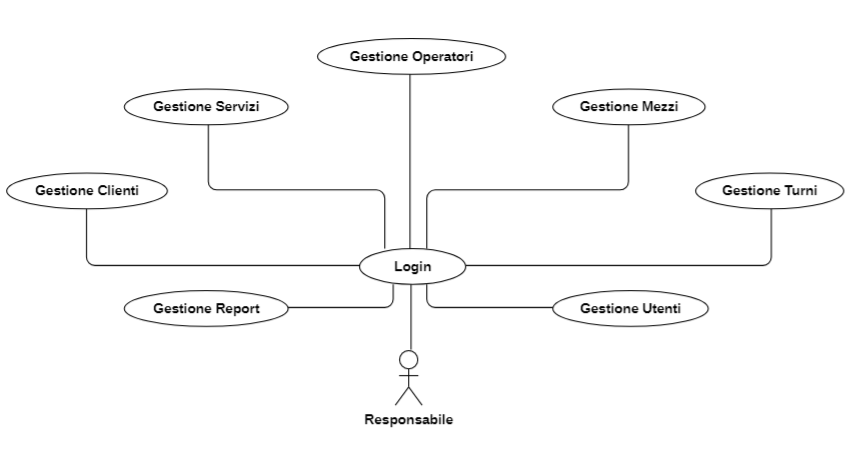
\includegraphics[scale=0.8]{UC_general}
	\caption{Diagramma generale dei casi d'uso}
\end{figure}
\newpage
\subsection{Gestione Operatori}
\begin{figure}[H]
	\centering
	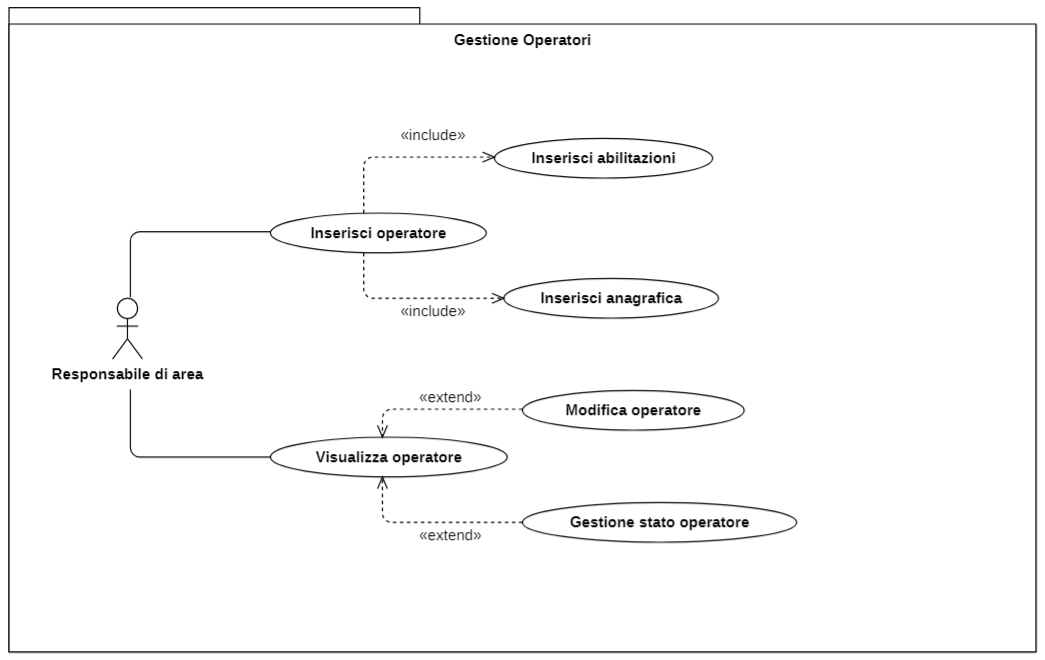
\includegraphics[scale=0.7]{UC_GestioneDipendenti}
	\caption{Diagramma dei casi d'uso - Gestione Operatori}
\end{figure}

\subsubsection{Caso d'uso: Inserisci Operatore}

Questo caso d’uso si verifica qualora il responsabile di area voglia inserire un nuovo operatore a sistema.\\
\textbf{Pre-Condizioni}\\
L’operatore non esiste nel sistema.\\
\textbf{Post-Condizioni}\\
Il nuovo operatore è stato inserito nel sistema (o si è verificata l’impossibilità di aggiungerlo).\\
\textbf{Sequenza eventi principale}
\begin{enumerate}
	\item Il caso d’uso inizia quando il responsabile di area vuole inserire le informazioni di un nuovo operatore.
	\item Il sistema visualizza la schermata di inserimento delle informazioni del nuovo operatore.
	\item Il responsabile di area fornisce tutte le informazioni richieste.
	\item Il responsabile di area avvia la procedura di inserimento di un nuovo operatore.
	\item Il sistema aggiunge con successo il nuovo operatore a sistema.
\end{enumerate}
\textbf{Sequenza degli eventi alternativa}\\
La sequenza alternativa inizia dal punto 4.
\begin{enumerate}
	\setcounter{enumi}{4}
	\item Le informazioni inserite dal responsabile di area sono incomplete o errate.
	\item L’inserimento del nuovo operatore fallisce.
\end{enumerate}
\newpage

\subsubsection{Caso d'uso Visualizza Operatore}

Questo caso d’uso si verifica qualora il responsabile di area voglia visualizzare le informazioni di un operatore.\\
\textbf{Pre-Condizioni}\\
L’operatore esiste nel sistema.\\
\textbf{Post-Condizioni}\\
Nessuna.\\
\textbf{Sequenza eventi principale}
\begin{enumerate}
	\item Il caso d’uso inizia quando il responsabile di area vuole visualizzare le informazioni di un operatore
	\item Il sistema legge le informazioni dell’operatore scelto dal responsabile di area.
	\item Il sistema visualizza a schermo le informazioni dell’operatore.
\end{enumerate}
\textbf{Sequenza degli eventi alternativa}\\
Nessuna.

\subsubsection{Caso d'uso: Modifica Dati Operatore}

Questo caso d’uso si verifica qualora il responsabile di area voglia modificare i dati di un operatore esistente nel sistema.\\
\textbf{Pre-Condizioni}\\
L’operatore esiste nel sistema.\\
\textbf{Post-Condizioni}\\
I dati dell'operatore sono stati modificati (o la modifica non è andata a buon fine).\\
\textbf{Sequenza eventi principale}
\begin{enumerate}
	\item Il caso d’uso inizia quando il responsabile di area vuole modificare le informazioni di un operatore.
	\item Il sistema legge le informazioni dell’operatore scelto dal responsabile di area.
	\item Il sistema visualizza a schermo le informazioni dell’operatore.
	\item Il responsabile di area avvia la procedura di modifica.
	\item Il sistema modifica dal sistema le informazioni dell’operatore.
\end{enumerate}
\textbf{Sequenza degli eventi alternativa}\\
Nessuna.

\subsubsection{Caso d'uso: Gestione Stato Operatore}

Questo caso d’uso si verifica qualora il responsabile di area voglia gestire i giorni in cui l’operatore è indisponibile (ferie/malattia). Nello stato dell’operatore è incluso anche il suo periodo di assunzione.\\
\textbf{Pre-Condizioni}\\
L'operatore esiste nel sistema.\\
\textbf{Post-Condizioni}\\
Lo stato dell'operatore è stato modificato (o si è verificata l’impossibilità di modificarlo).\\
\textbf{Sequenza eventi principale}
\begin{enumerate}
	\item Il caso d’uso inizia quando il responsabile di area vuole visualizzare le informazioni dello stato di un operatore.
	\item Il sistema legge le informazioni dello stato dell’operatore scelto dal responsabile di area.
	\item Il sistema visualizza a schermo le informazioni dello stato dell’operatore.
	\item Il responsabile di area avvia la procedura di modifica dei giorni nel quale l’operatore avrebbe dovuto lavorare.
	\item Il sistema aggiorna le informazioni dello stato dell’operatore.
\end{enumerate}
\textbf{Sequenza degli eventi alternativa}\\
La sequenza alternativa inizia dal punto 4.
\begin{enumerate}
	\setcounter{enumi}{4}
	\item Le modifiche effettuate dal responsabile di area non sono corrette.
	\item La modifica dello stato dell'operatore fallisce.
\end{enumerate}
\newpage


%-----------------------------------GESIONE MEZZI----------------------------------------------------
\subsection{Gestione Mezzi}
\begin{figure}[H]
	\centering
	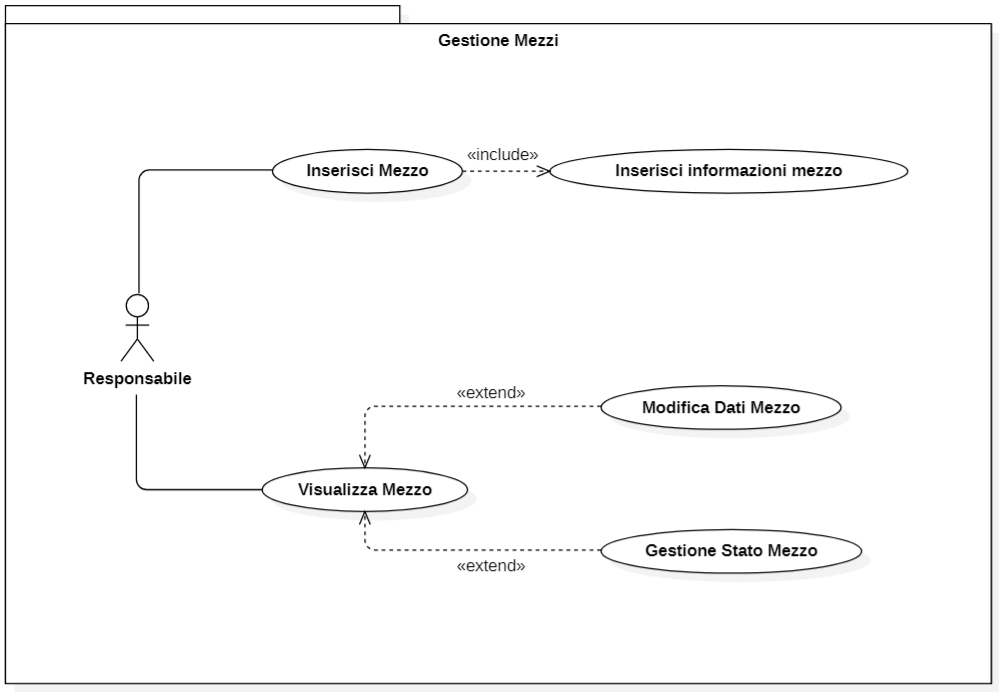
\includegraphics[scale=0.7]{UC_GestioneMezzi}
	\caption{Diagramma dei casi d'uso - Gestione Mezzi}
\end{figure}

\subsubsection{Caso d'uso: Inserisci Mezzo}

Questo caso d’uso si verifica qualora il responsabile di area voglia inserire un nuovo mezzo a sistema.\\
\textbf{Pre-Condizioni}\\
Il mezzo non esiste nel sistema.\\
\textbf{Post-Condizioni}\\
Il nuovo mezzo è stato inserito nel sistema (o si è verificata l’impossibilita di aggiungerlo).\\
\textbf{Sequenza eventi principale}
\begin{enumerate}
	\item Il caso d’uso inizia quando il responsabile di area vuole inserire le informazioni di un nuovo dipendente.
	\item Il sistema visualizza la schermata di inserimento delle informazioni del nuovo mezzo.
	\item Il responsabile di area fornisce tutte le informazioni richieste.
	\item Il responsabile di area avvia la procedura di inserimento di un nuovo mezzo.
	\item Il sistema aggiunge con successo il nuovo mezzo a sistema.
\end{enumerate}
\textbf{Sequenza degli eventi alternativa}\\
La sequenza alternativa inizia dal punto 4.
\begin{enumerate}
	\setcounter{enumi}{4}
	\item Le informazioni inserite dal responsabile di area sono incomplete o errate.
	\item L’inserimento del nuovo mezzo fallisce.
\end{enumerate}
\newpage

\subsubsection{Caso d'uso: Visualizza Mezzo}

Questo caso d’uso si verifica qualora il responsabile di area voglia visualizzare le informazioni di un mezzo.\\
\textbf{Pre-Condizioni}\\
Il mezzo esiste nel sistema.\\
\textbf{Post-Condizioni}\\
Nessuna.\\
\textbf{Sequenza eventi principale}
\begin{enumerate}
	\item Il caso d’uso inizia quando il responsabile di area vuole visualizzare le informazioni di un mezzo.
	\item Il sistema legge le informazioni del mezzo scelto dal responsabile di area.
	\item Il sistema visualizza a schermo le informazioni del mezzo.
\end{enumerate}
\textbf{Sequenza degli eventi alternativa}\\
Nessuna.

\subsubsection{Caso d'uso: Modifica Dati Mezzo}

Questo caso d’uso si verifica qualora il responsabile di area voglia modificare le informazioni di un mezzo esistente nel sistema.\\
\textbf{Pre-Condizioni}\\
Il  mezzo esiste nel sistema.\\
\textbf{Post-Condizioni}\\
I dati del mezzo sono stati modificati.\\
\textbf{Sequenza eventi principale}
\begin{enumerate}
	\item Il caso d’uso inizia quando il responsabile di area vuole modificare un mezzo.
	\item Il sistema legge le informazioni del mezzo scelto dal responsabile di area.
	\item Il sistema visualizza a schermo le informazioni del mezzo.
	\item Il responsabile di area avvia la procedura di modifica.
	\item Il sistema modifica dal sistema le informazioni del mezzo.
\end{enumerate}
\textbf{Sequenza degli eventi alternativa}\\
Nessuna.

\subsubsection{Caso d'uso: Gestione Stato Mezzo}

Questo caso d’uso si verifica qualora il responsabile di area voglia gestire i giorni in cui il mezzo è indisponibile.\\
\textbf{Pre-Condizioni}\\
Il mezzo esiste nel sistema.\\
\textbf{Post-Condizioni}\\
Lo stato del mezzo è stato modificato (o si è verificata l’impossibilità di modificarlo).\\
\textbf{Sequenza eventi principale}
\begin{enumerate}
	\item Il caso d’uso inizia quando il responsabile di area vuole visualizzare le informazioni di un mezzo.
	\item Il sistema legge le informazioni del mezzo scelto dal responsabile di area.
	\item Il sistema visualizza a schermo le informazioni del mezzo.
	\item Il responsabile di area avvia la procedura di modifica dei giorni durante i quali il mezzo doveva essere utilizzato.
	\item Il sistema aggiorna le informazioni del mezzo.
\end{enumerate}
\textbf{Sequenza degli eventi alternativa}\\
La sequenza alternativa inizia dal punto 4.
\begin{enumerate}
	\setcounter{enumi}{4}
	\item Le modifiche effettuate dal responsabile di area non sono corrette.
	\item La modifica dello stato del mezzo fallisce
\end{enumerate}
\newpage

\subsection{Gestione Servizi}
\begin{figure}[H]
	\centering
	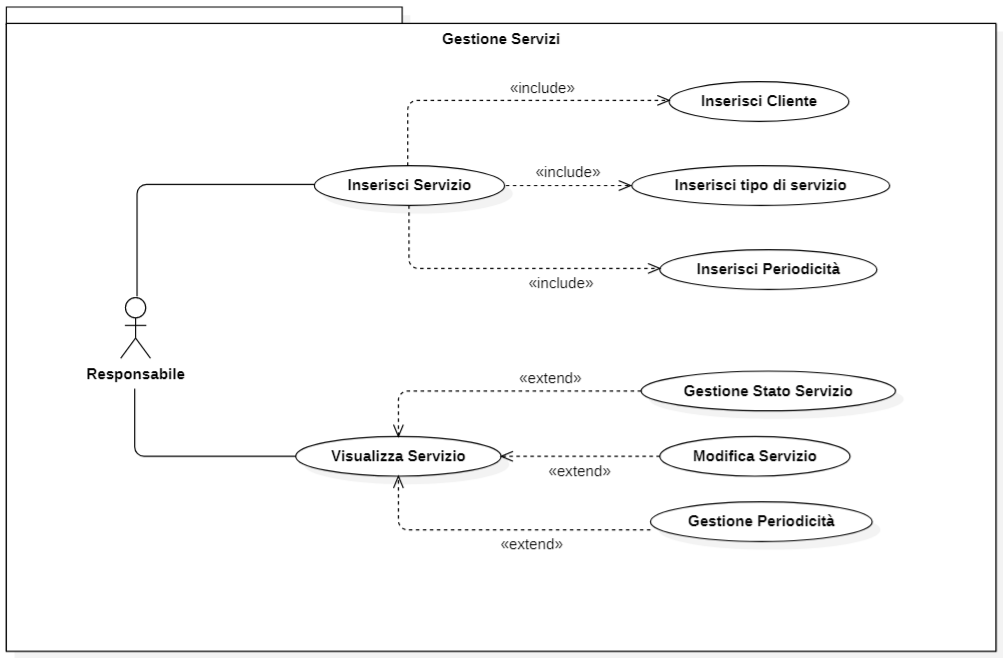
\includegraphics[scale=0.7]{UC_GestioneServizi}
	\caption{Diagramma dei casi d'uso - Gestione Servizi}
\end{figure}

\subsubsection{Caso d'uso: Inserisci Servizio}

Questo caso d’uso si verifica qualora il responsabile di area voglia inserire un nuovo servizio a sistema.\\
\textbf{Pre-Condizioni}\\
Il servizio non esiste nel sistema.\\
\textbf{Post-Condizioni}\\
Il nuovo servizio è stato inserito nel sistema (o si è verificata l’impossibilita di aggiungerlo).\\
\textbf{Sequenza eventi principale}
\begin{enumerate}
	\item Il caso d’uso inizia quando il responsabile di area vuole inserire le informazioni di un nuovo servizio.
	\item Il sistema visualizza la schermata di inserimento delle informazioni del nuovo servizio.
	\item Il responsabile di area fornisce tutte le informazioni richieste.
	\item Il responsabile di area avvia la procedura di inserimento di un nuovo servizio.
	\item l sistema aggiunge con successo il nuovo servizio a sistema.
\end{enumerate}
\textbf{Sequenza degli eventi alternativa}\\
La sequenza alternativa inizia dal punto 4.
\begin{enumerate}
	\setcounter{enumi}{4}
	\item Le informazioni inserite dal responsabile di area sono incomplete o errate.
	\item L’inserimento del nuovo servizio fallisce.
\end{enumerate}
\newpage

\subsubsection{Caso d'uso: Visualizza Servizio}

Questo caso d’uso si verifica qualora il responsabile di area voglia visualizzare le informazioni di un servizio.\\
\textbf{Pre-Condizioni}\\
Il servizio esiste nel sistema.\\
\textbf{Post-Condizioni}\\
Nessuna.\\
\textbf{Sequenza eventi principale}
\begin{enumerate}
	\item Il caso d’uso inizia quando il responsabile di area vuole visualizzare le informazioni di un servizio.
	\item Il sistema legge le informazioni del servizio scelto dal responsabile di area.
	\item Il sistema visualizza a schermo le informazioni del servizio.
\end{enumerate}
\textbf{Sequenza degli eventi alternativa}\\
Nessuna.

\subsubsection{Caso d'uso: Modifica Servizio}

Questo caso d’uso si verifica qualora il responsabile di area voglia modificare le informazioni di un servizio esistente nel sistema.\\
\textbf{Pre-Condizioni}\\
Il servizio esiste nel sistema.\\
\textbf{Post-Condizioni}\\
Le informazioni sul servizio sono state modificate.\\
\textbf{Sequenza eventi principale}
\begin{enumerate}
	\item Il caso d’uso inizia quando il responsabile di area vuole modificare i dati di un servizio.
	\item Il sistema legge le informazioni del servizio scelto dal responsabile di area.
	\item Il sistema visualizza a schermo le informazioni del servizio.
	\item Il responsabile di area avvia la procedura di modifica.
	\item Il sistema modifica dal sistema le informazioni del servizio.
\end{enumerate}
\textbf{Sequenza degli eventi alternativa}\\
Nessuna.
\newpage

\subsubsection{Caso d'uso: Gestione Stato Servizio}

Questo caso d’uso si verifica qualora il responsabile di area voglia annullare o modificare un servizio stabilito in un determinato giorno a causa di un imprevisto.\\
\textbf{Pre-Condizioni}\\
Il servizio esiste nel sistema.\\
\textbf{Post-Condizioni}\\
Lo stato del servizio è stato modificato (o si è verificata)\\
\textbf{Sequenza eventi principale}
\begin{enumerate}
	\item Il caso d’uso inizia quando il responsabile di area vuole visualizzare le informazioni di un servizio.
	\item Il sistema legge le informazioni del servizio scelto dal responsabile di area.
	\item Il sistema visualizza a schermo le informazioni del servizio.
	\item Il responsabile di area avvia la procedura di modifica o di annullamento.
	\item Il sistema aggiorna le informazioni del servizio.
\end{enumerate}
\textbf{Sequenza degli eventi alternativa}\\
La sequenza alternativa inizia dal punto 4.
\begin{enumerate}
	\setcounter{enumi}{4}
	\item Le modifiche effettuate dal responsabile di area non sono corrette.
	\item La modifica dello stato del servizio fallisce.
\end{enumerate}

\subsubsection{Caso d'uso: Gestione Periodicità}
Questo caso d’uso si verifica qualora il responsabile di area voglia modificare la cadenza (ogni quanto tempo si ripete lo svolgimento) di un servizio.\\
\textbf{Pre-Condizioni}\\
Il servizio esiste nel sistema.\\
\textbf{Post-Condizioni}\\
La periodicità del servizio è stata modificata (o si è verificata l’impossibilità di modificarla).\\
\textbf{Sequenza eventi principale}
\begin{enumerate}
	\item Il caso d’uso inizia quando il responsabile di area vuole visualizzare le informazioni di un servizio.
	\item Il sistema legge le informazioni del servizio scelto dal responsabile di area.
	\item Il sistema visualizza a schermo le informazioni del servizio.
	\item Il responsabile di area avvia la procedura di modifica.
	\item Il sistema aggiorna le informazioni del servizio.
\end{enumerate}
\textbf{Sequenza degli eventi alternativa}\\
La sequenza alternativa inizia dal punto 4.
\begin{enumerate}
	\setcounter{enumi}{4}
	\item Le modifiche effettuate dal responsabile di area non sono corrette.
	\item La modifica della periodicità fallisce.
\end{enumerate}
\newpage

\subsection{Gestione Clienti}
\begin{figure}[H]
	\centering
	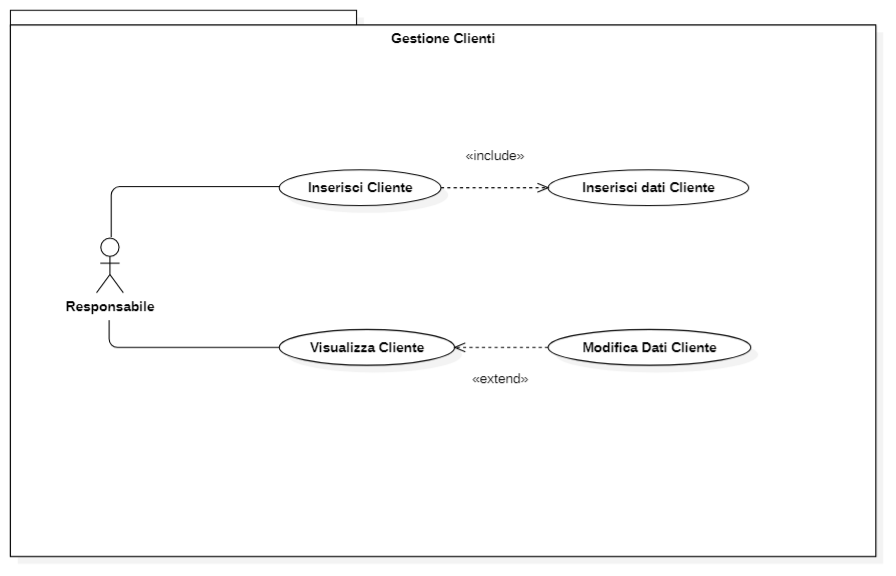
\includegraphics[scale=0.7]{UC_GestioneClienti}
	\caption{Diagramma dei casi d'uso - Gestione Clienti}
\end{figure}

\subsubsection{Caso d'uso: Inserisci Cliente}

Questo caso d’uso si verifica qualora il responsabile di area voglia inserire un nuovo cliente a sistema.\\
\textbf{Pre-Condizioni}\\
Il cliente non esiste nel sistema\\
\textbf{Post-Condizioni}\\
Il nuovo cliente è stato inserito nel sistema (o si è verificata l’impossibilita di aggiungerlo)\\
\textbf{Sequenza eventi principale}
\begin{enumerate}
	\item Il caso d’uso inizia quando il responsabile di area vuole inserire le informazioni di un nuovo cliente.
	\item Il sistema visualizza la schermata di inserimento delle informazioni del nuovo cliente.
	\item Il responsabile di area fornisce tutte le informazioni richieste.
	\item Il responsabile di area avvia la procedura di inserimento di un nuovo cliente.
	\item Il sistema aggiunge con successo il nuovo cliente a sistema.
\end{enumerate}
\textbf{Sequenza degli eventi alternativa}\\
La sequenza alternativa inizia dal punto 4.
\begin{enumerate}
	\item Le informazioni inserite dal responsabile di area sono incomplete o errate.
	\item L’inserimento del nuovo cliente fallisce.
\end{enumerate}
\newpage

\subsubsection{Caso d'uso: Visualizza Cliente}

Questo caso d’uso si verifica qualora il responsabile di area voglia visualizzare le informazioni di un cliente.\\
\textbf{Pre-Condizioni}\\
Il cliente esiste nel sistema.\\
\textbf{Post-Condizioni}\\
Nessuna.\\
\textbf{Sequenza eventi principale}
\begin{enumerate}
	\item Il caso d’uso inizia quando il responsabile di area vuole visualizzare le informazioni di un cliente.
	\item Il sistema legge le informazioni del cliente scelto dal responsabile di area.
	\item Il sistema visualizza a schermo le informazioni del cliente.
\end{enumerate}
\textbf{Sequenza degli eventi alternativa}\\
Nessuna.

\subsubsection{Caso d'uso: Modifica Dati Cliente}

Questo caso d’uso si verifica qualora il responsabile di area voglia modificare le informazioni di un cliente esistente nel sistema.\\
\textbf{Pre-Condizioni}\\
Il cliente esiste nel sistema.\\
\textbf{Post-Condizioni}\\
I dati del cliente sono stati modificati.\\
\textbf{Sequenza eventi principale}
\begin{enumerate}
	\item Il caso d’uso inizia quando il responsabile di area vuole modificare i dati di un cliente.
	\item Il sistema legge le informazioni del cliente scelto dal responsabile di area.
	\item Il sistema visualizza a schermo le informazioni del cliente.
	\item Il responsabile di area avvia la procedura di modifica.
	\item Il sistema modifica dal sistema le informazioni del cliente.
\end{enumerate}
\textbf{Sequenza degli eventi alternativa}\\
Nessuna.
\newpage

\subsection{Gestione Turni}
\begin{figure}[H]
	\centering
	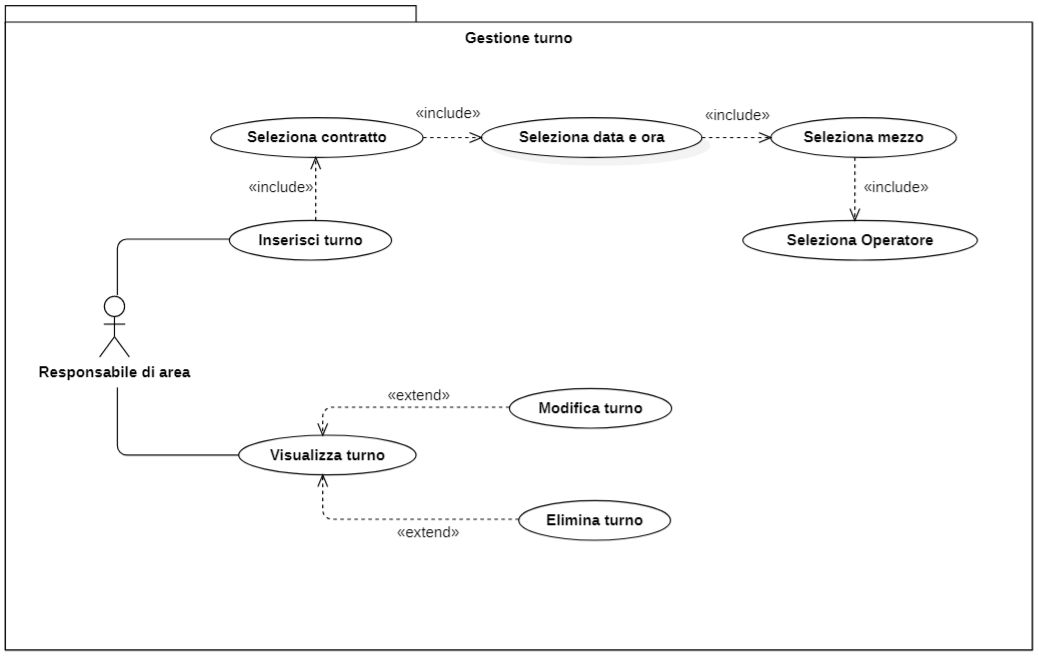
\includegraphics[scale=0.7]{UC_GestioneTurni}
	\caption{Diagramma dei casi d'uso - Gestione Turni}
\end{figure}

\subsubsection{Caso d'uso: Inserisci Turno}

Questo caso d’uso si verifica qualora il responsabile di area voglia inserire un nuovo turno a sistema.\\
\textbf{Pre-Condizioni}\\
Il turno non esiste nel sistema.\\
\textbf{Post-Condizioni}\\
Il turno è stato inserito nel sistema.\\
\textbf{Sequenza eventi principale}
\begin{enumerate}
	\item Il caso d’uso inizia quando il responsabile di area vuole inserire un nuovo turno.
    \item Il sistema visualizza la schermata di inserimento delle informazioni del nuovo turno.
	\item Il responsabile di area fornisce tutte le informazioni richieste.
	\item Il responsabile di area avvia la procedura di inserimento di un nuovo turno.
	\item Il sistema aggiunge con successo il nuovo turno a sistema.
\end{enumerate}
\textbf{Sequenza degli eventi alternativa}\\
Nessuna.
\newpage

\subsubsection{Cado d'uso: Visualizza Turno}

Questo caso d’uso si verifica qualora il responsabile di area voglia visualizzare le informazioni di un turno.\\
\textbf{Pre-Condizioni}\\
Il turno esiste nel sistema.\\
\textbf{Post-Condizioni}\\
Nessuna.\\
\textbf{Sequenza eventi principale}
\begin{enumerate}
	\item Il caso d’uso inizia quando il responsabile di area vuole visualizzare le informazioni di un turno.
	\item Il sistema legge le informazioni del turno scelto dal responsabile di area.
	\item Il sistema visualizza a schermo le informazioni del turno scelto dal responsabile di area.
\end{enumerate}
\textbf{Sequenza degli eventi alternativa}\\
Nessuna.

\subsubsection{Caso d’uso: Modifica Turno}

Questo caso d’uso si verifica qualora il responsabile di area voglia modificare le informazioni di un turno esistente nel sistema.\\
\textbf{Pre-Condizioni}\\
Il turno esiste nel sistema.\\
\textbf{Post-Condizioni}\\
Il turno è stato modificato.\\
\textbf{Sequenza eventi principale}\\
\begin{enumerate}
    \item Il caso d’uso inizia quando il responsabile di area vuole modificare un turno.
	\item Il sistema legge le informazioni del turno scelto dal responsabile di area.
	\item Il sistema visualizza a schermo le informazioni del turno.
	\item Il responsabile di area avvia la procedura di modifica.
	\item Il sistema modifica dal sistema le informazioni del turno.
\end{enumerate}
\textbf{Sequenza degli eventi alternativa}\\
Nessuna.

\subsection{Caso d'uso: Elimina Turno}

Questo caso d’uso si verifica qualora il responsabile di area voglia eliminare un turno dal sistema.\\
\textbf{Pre-Condizioni}\\
Il turno esiste nel sistema.\\
\textbf{Post-Condizioni}\\
Il turno non esiste più nel sistema.\\
\textbf{Sequenza eventi principale}
\begin{enumerate}
	\item Il caso d’uso inizia quando il responsabile di area vuole eliminare un turno dal sistema.
	\item Il sistema legge le informazioni del turno scelto dal responsabile di area.
	\item Il sistema visualizza a schermo le informazioni del turno.
	\item Il responsabile d’area avvia la procedura d’eliminazione.
	\item Il sistema elimina il turno dal sistema.
\end{enumerate}
\textbf{Sequenza degli eventi alternativa}\\
Nessuna.
\newpage

\subsection{Gestione Utenti}
\begin{figure}[H]
	\centering
	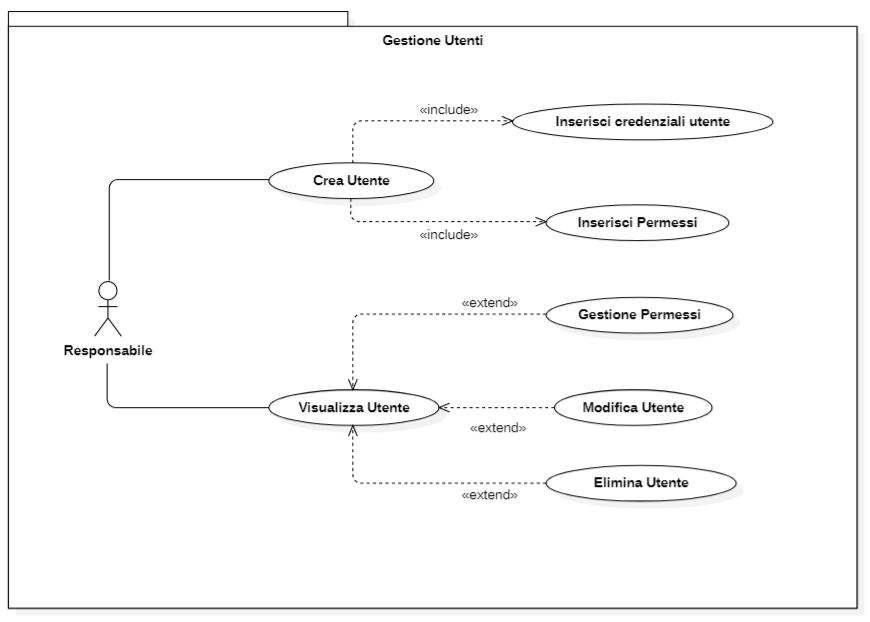
\includegraphics[scale=0.7]{UC_GestioneUtenti}
	\caption{Diagramma dei casi d'uso - Gestione Utenti}
\end{figure}

\subsubsection{Caso d'uso: Crea Utente}

Questo caso d’uso si verifica qualora il responsabile di area voglia creare un nuovo utente a sistema.\\
\textbf{Pre-Condizioni}\\
L’utente non esiste nel sistema.\\
\textbf{Post-Condizioni}\\
Il nuovo utente è stato inserito nel sistema(o si è verificata l’impossibilita di crearlo).\\
\textbf{Sequenza eventi principale}\\
\begin{enumerate}
	\item Il caso d’uso inizia quando il responsabile di area vuole creare un nuovo utente.
	\item Il sistema visualizza la schermata di inserimento delle credenziali e dei permessi del nuovo utente.
	\item Il responsabile di area fornisce tutte le credenziali e i permessi richiesti.
	\item Il responsabile di area avvia la procedura di creazione di un nuovo utente.
	\item Il sistema crea con successo il nuovo utente a sistema.
\end{enumerate}
\textbf{Sequenza degli eventi alternativa}\\
La sequenza alternativa inizia dal punto 4.
\begin{enumerate}
	\setcounter{enumi}{4}
	\item Le credenziali e i permessi inseriti dal responsabile di area sono incompleti o errati.
	\item La creazione del nuovo utente fallisce.
\end{enumerate}
\newpage

\subsubsection{Caso d'uso: Visualizza Utente}

Questo caso d’uso si verifica qualora il responsabile di area voglia visualizzare le credenziali e i permessi di un utente.\\
\textbf{Pre-Condizioni}\\
L’utente esiste nel sistema.\\
\textbf{Post-Condizioni}\\
Nessuna.\\
\textbf{Sequenza eventi principale}\\
\begin{enumerate}
	\item Il caso d’uso inizia quando il responsabile di area vuole visualizzare le credenziali e i permessi di un utente.
	\item Il sistema legge le credenziali e i permessi dell’utente scelto dal responsabile di area.
	\item Il sistema visualizza a schermo le credenziali e i permessi dell’utente.
\end{enumerate}
\textbf{Sequenza degli eventi alternativa}\\
Nessuna.

\subsubsection{Caso d'uso: Gestione Permessi}

Questo caso d’uso si verifica qualora il responsabile di area voglia visualizzare quali parti di software saranno utilizzabili da un determinato utente.\\
\textbf{Pre-Condizioni}\\
L'utente esiste nel sistema.\\
\textbf{Post-Condizioni}\\
Nessuna.\\
\textbf{Sequenza eventi principale}\\
\begin{enumerate}
	\item Il caso d’uso inizia quando il responsabile di area vuole visualizzare il modulo accessibile ad un determinato utente.
	\item Il sistema legge le informazioni dell’utente scelto dal responsabile di area.
	\item Il sistema visualizza a schermo il modulo accessibile all’utente scelto.
\end{enumerate}
\textbf{Sequenza degli eventi alternativa}\\
Nessuna.

\subsubsection{Caso d'uso: Elimina Utente}

Questo caso d’uso si verifica qualora il responsabile di area voglia eliminare un utente dal sistema.\\
\textbf{Pre-Condizioni}\\
L’utente esiste nel sistema.\\
\textbf{Post-Condizioni}\\
L’utente non esiste più nel sistema.\\
\textbf{Sequenza eventi principale}
\begin{enumerate}
	\item Il caso d’uso inizia quando il responsabile di area vuole eliminare un utente dal sistema.
	\item Il sistema legge le credenziali e i permessi dell’utente scelto dal responsabile di area.
	\item Il sistema visualizza a schermo le credenziali e i permessi dell’utente.
	\item Il responsabile d’area avvia la procedura d’eliminazione.
	\item Il sistema elimina l’utente dal sistema.
\end{enumerate}
\textbf{Sequenza degli eventi alternativa}\\
Nessuna.\\

\subsection{Gestione Report}
\begin{figure}[H]
	\centering
	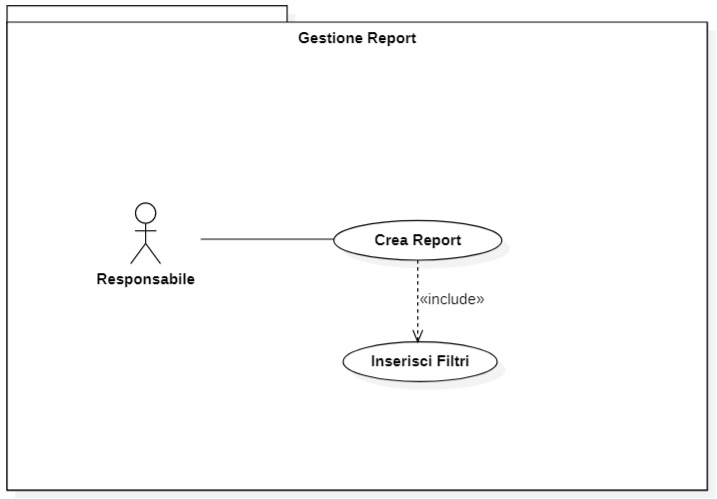
\includegraphics[scale=0.7]{UC_GestioneReport}
	\caption{Diagramma dei casi d'uso - Gestione Report}
\end{figure}

\subsubsection{Caso d’uso: Crea Report}

Questo caso d’uso si verifica qualora il responsabile di area voglia creare un report.\\
\textbf{Pre-Condizioni}\\
Nessuna.\\
\textbf{Post-Condizioni}\\
Nessuna.\\
\textbf{Sequenza eventi principale}
\begin{enumerate}
	\item Il caso d’uso inizia quando il responsabile di area vuole creare un report.
	\item Il responsabile di Area inserisce i filtri sulle informazione che il report deve contenere.
	\item Il sistema crea il report.
\end{enumerate}
\textbf{Sequenza degli eventi alternativa}\\
Nessuna.

\subsubsection{Caso d'uso: Visualizza Report}

Questo caso d'uso si verifica dopo che il responsabile di area ha creato un report e vuole visualizzarlo.\\
\textbf{Pre-Condizioni}\\
Il sistema ha creato il report in precedenza.\\
\textbf{Post-Condizioni}\\
Nessuna
\textbf{Sequenza eventi principale}
\begin{enumerate}
	\item Il caso d'uso si verifica quando il responsabile di area vuole visualizzare un Report.
	\item Il sistema visualizza le informazioni del report creato.
\end{enumerate}
\textbf{Sequenza degli eventi alternativa}\\
Nessuna.
\newpage

{
\begin{landscape}
\subsection{Matrice di Mapping}
Una volta progettati i diagrammi dei casi d'uso, attraverso la matrice di mapping possiamo verificare che ogni requisito sia soddisfatto da almeno un caso d'uso.
\scriptsize
\begin{figure}[H]
	\centering
	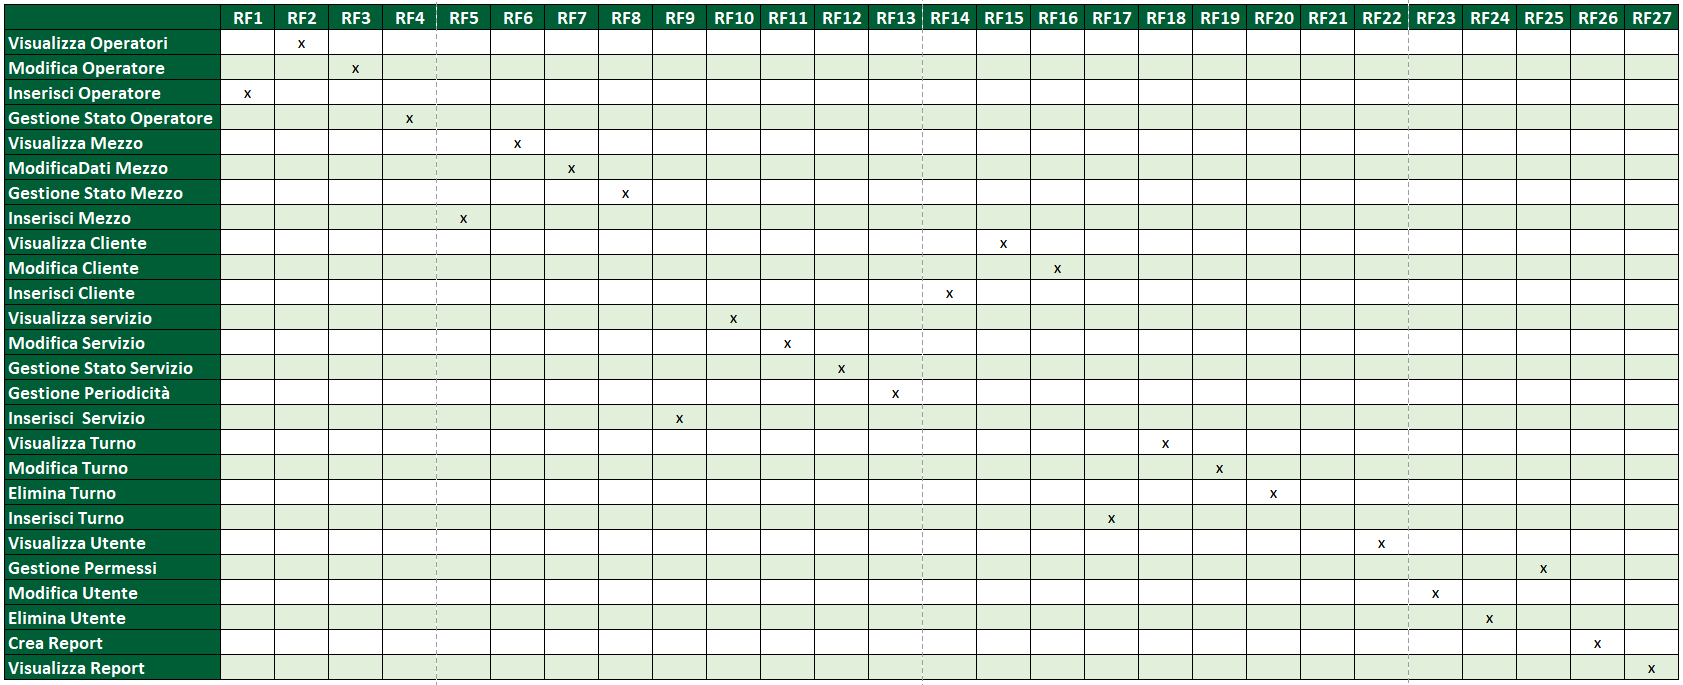
\includegraphics[scale=0.65]{matrice_mapping}
	\caption{Matrice di mapping}
\end{figure}
\end{landscape}
}

\section{Architettura}

Il pattern architetturale utilizzato per progettare il software è l'MVC(Model-View-Controller). La principale motivazione dietro questa scelta è la possibilità di separare la business logic del servizio dalle viste degli utenti, che, come emerso dall'intervista, abbiamo visto essere eterogenee; questo permette a diversi client di utilizzare lo stesso EDM(Enterprise Data Model), portando quindi ad un importante risparmio
di risorse. Per ora l'unica interfaccia che progetteremo è quella per un client desktop, sviluppata utilizzando il toolkit QT, senza quindi sfruttare appieno il potenziale di questo pattern, ma tenendo in considerazione un possibile sviluppo futuro di una web app legata al servizio.

Questo pattern divide il nostro servizio in due layers, ovvero il Presentation Layer ed il Model Layer:
Il Presentation Layer si occupa di mostrare le informazione all'utente e permette di visualizzare le interazioni con il programma.
Il Model Layer è responsabile della memorizzazione dei dati.
\\
\begin{figure}[H]
	\centering
	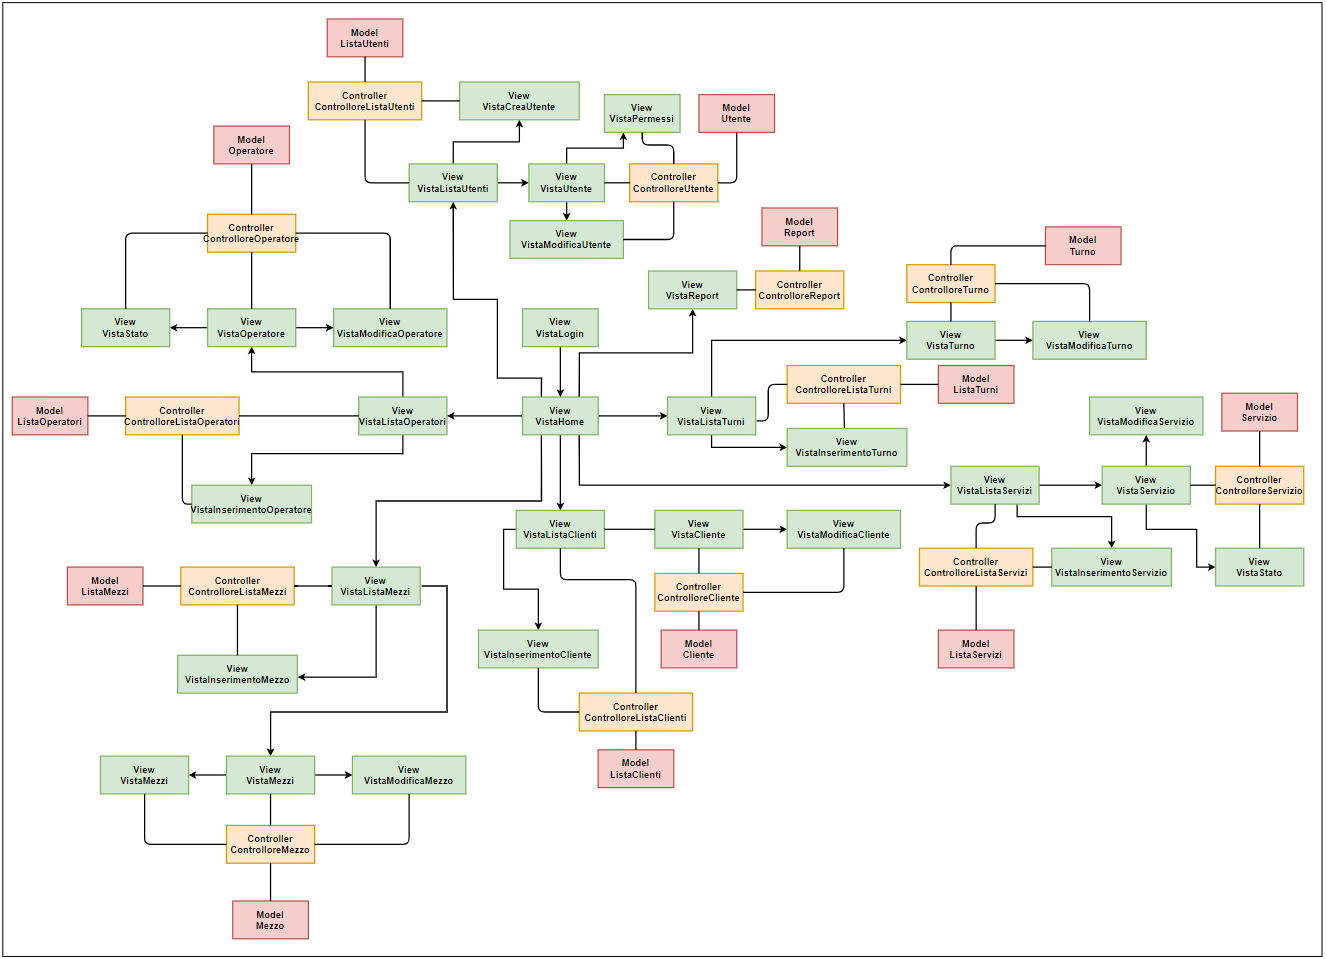
\includegraphics[scale=0.53]{Architettura}
	\caption{Schema architetturale}
\end{figure}

\newpage
\section{Diagramma delle classi}
Una volta progettati i diagrammi dei casi d'uso, attraverso la matrice di mapping possiamo verificare che ogni requisito sia soddisfatto da almeno un caso d'uso.
\\
\begin{figure}[H]
	\centering
	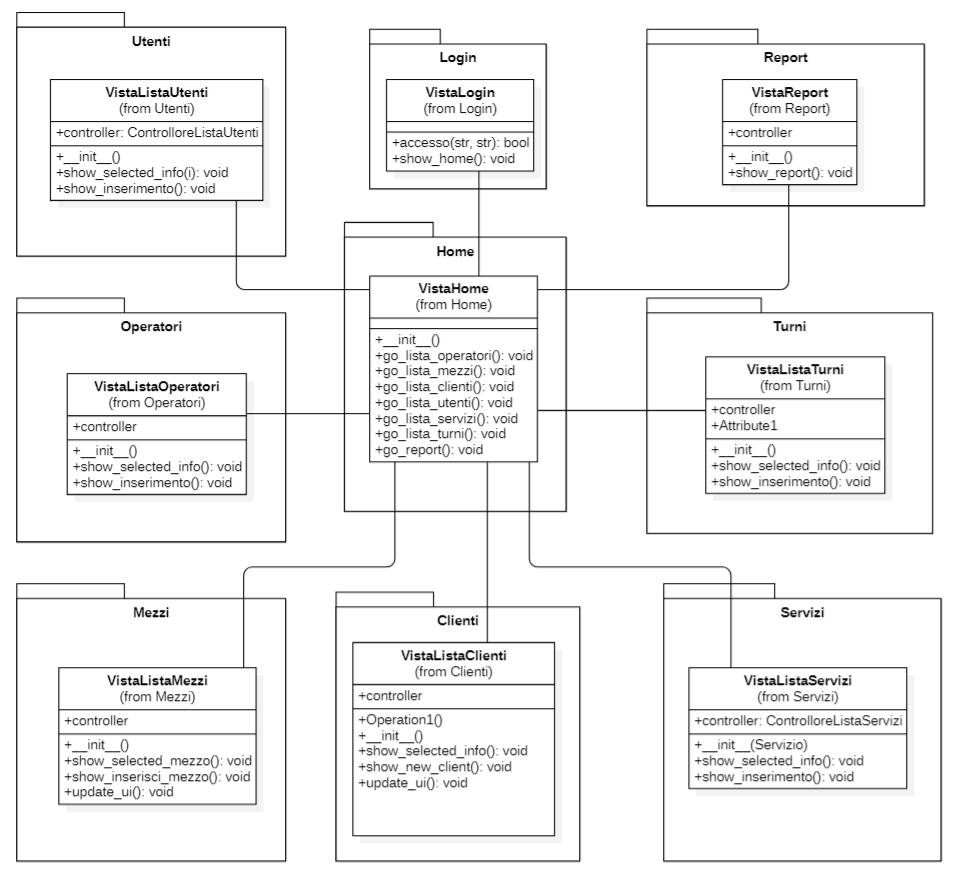
\includegraphics[scale=0.75]{classi_generale}
	\caption{Diagramma delle classi - Generale}
\end{figure}
\newpage

\subsection{Gestione Operatori}
\begin{figure}[H]
	\centering
	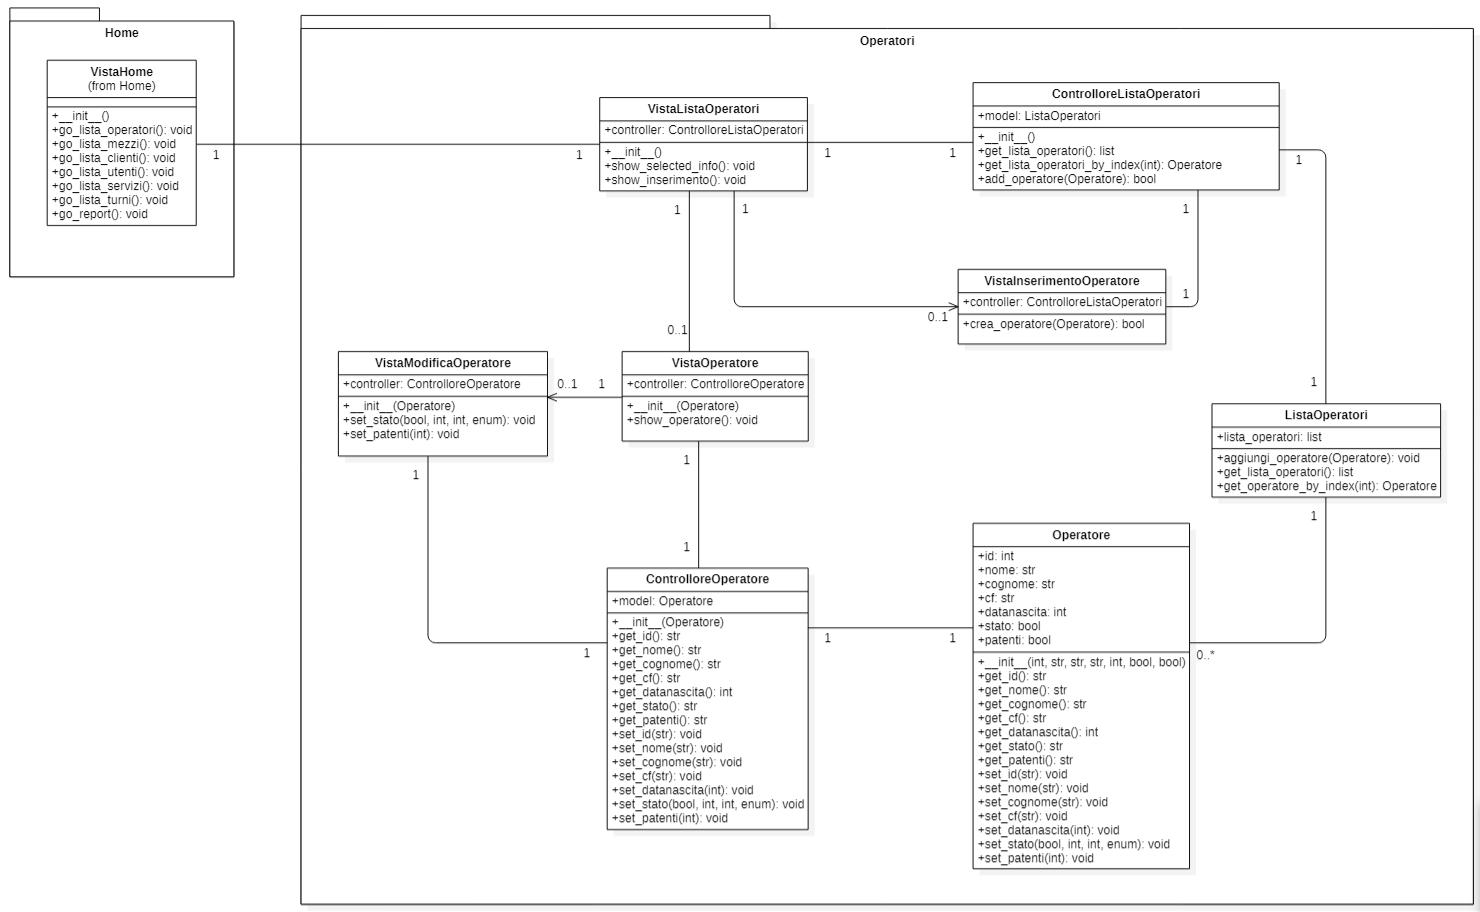
\includegraphics[scale=0.55]{classi_operatori}
	\caption{Diagramma delle classi - Operatori}
\end{figure}
\subsection{Gestione Mezzi}
\begin{figure}[H]
	\centering
	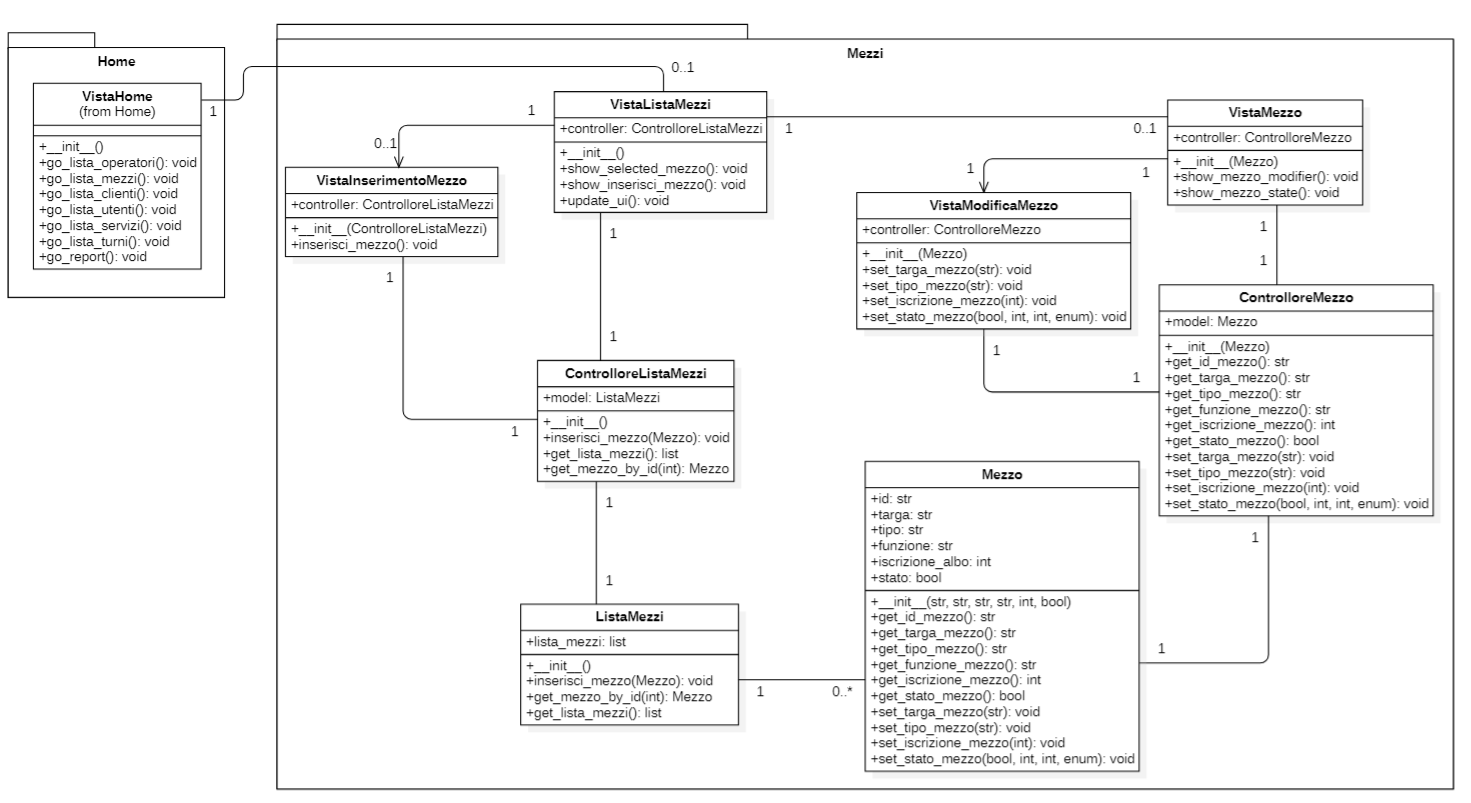
\includegraphics[scale=0.55]{classi_mezzi}
	\caption{Diagramma delle classi - Mezzi}
\end{figure}
\newpage

\subsection{Gestione Servizi}
\begin{figure}[H]
	\centering
	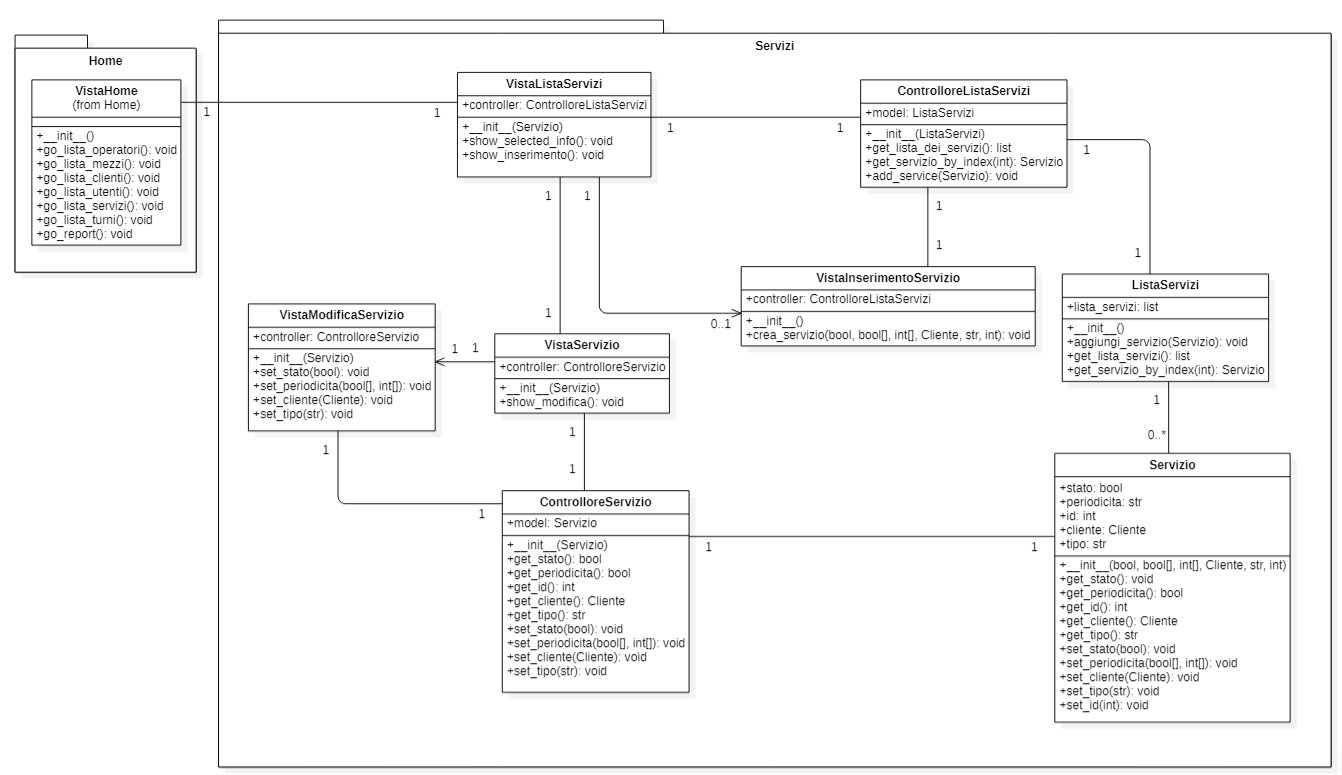
\includegraphics[scale=0.6]{classi_servizi}
	\caption{Diagramma delle classi - Servizi}
\end{figure}
\subsection{Gestione Turni}
\begin{figure}[H]
	\centering
	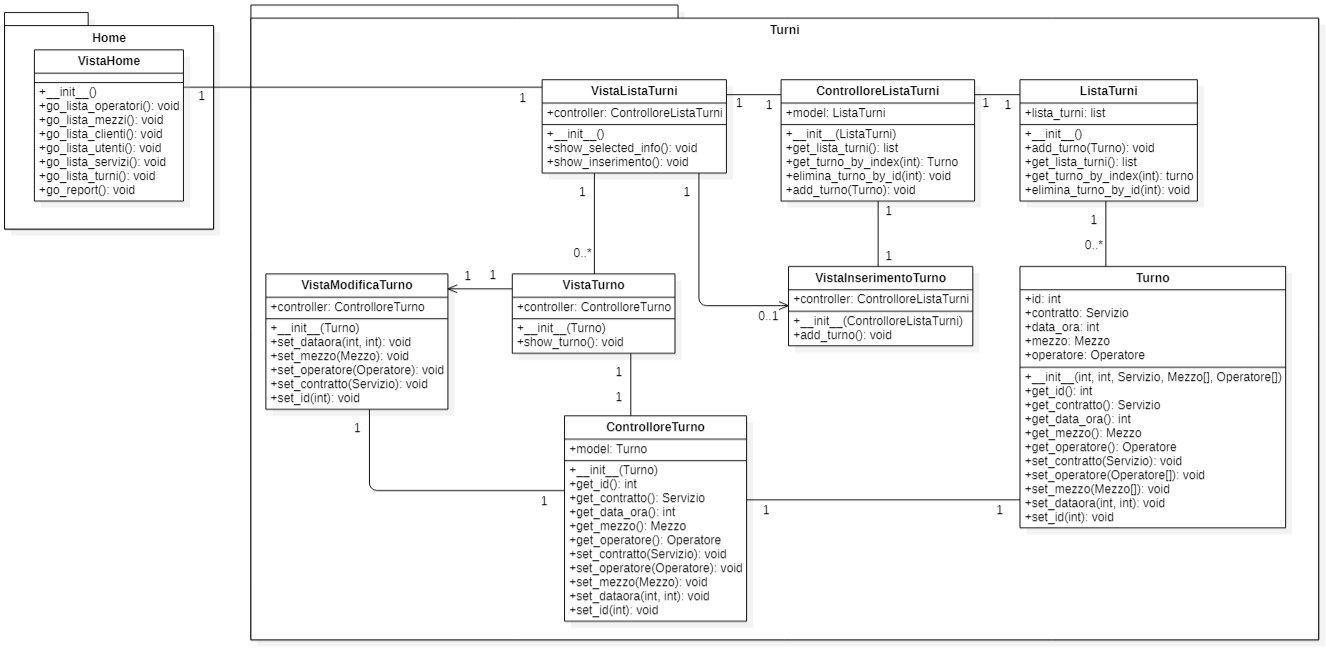
\includegraphics[scale=0.6]{classi_turni}
	\caption{Diagramma delle classi - Turni}
\end{figure}
\newpage

\subsection{Gestione Clienti}
\begin{figure}[H]
	\centering
	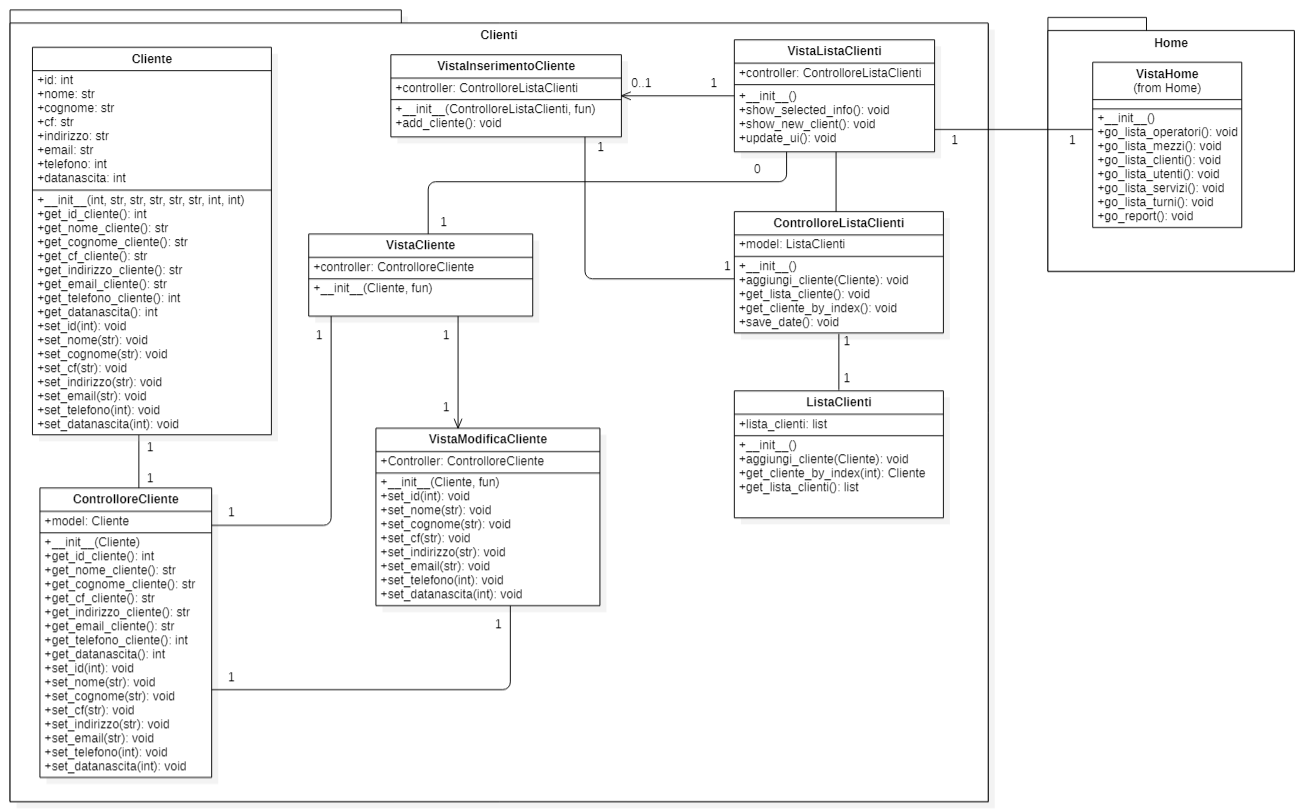
\includegraphics[scale=0.6]{classi_clienti}
	\caption{Diagramma delle classi - Clienti}
\end{figure}
\subsection{Gestione Utenti}
\begin{figure}[H]
	\centering
	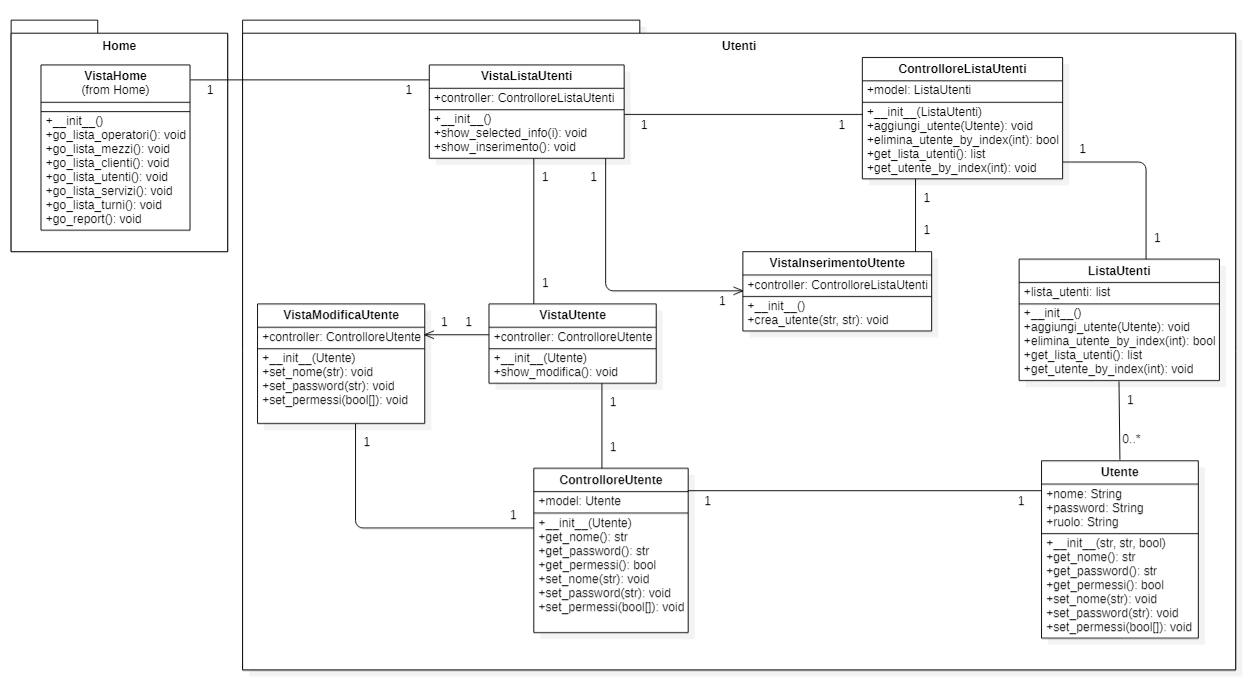
\includegraphics[scale=0.65]{classi_utenti}
	\caption{Diagramma delle classi - Utenti}
\end{figure}
\newpage

\subsection{Gestione Report}
\begin{figure}[H]
	\centering
	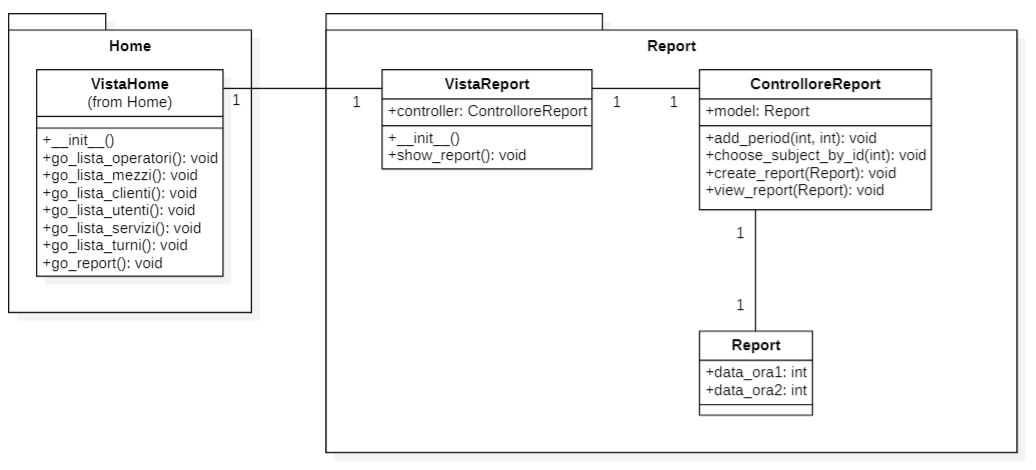
\includegraphics[scale=0.7]{classi_report}
	\caption{Diagramma delle classi - Report}
\end{figure}
\newpage

\section{Diagrammi delle sequenze}
I diagrammi delle sequenze vengono riportati solo in parte, in quanto molte delle attività prevedono azioni simili tra loro.
\subsection{Eliminazione Turno}
\begin{figure}[H]
	\centering
	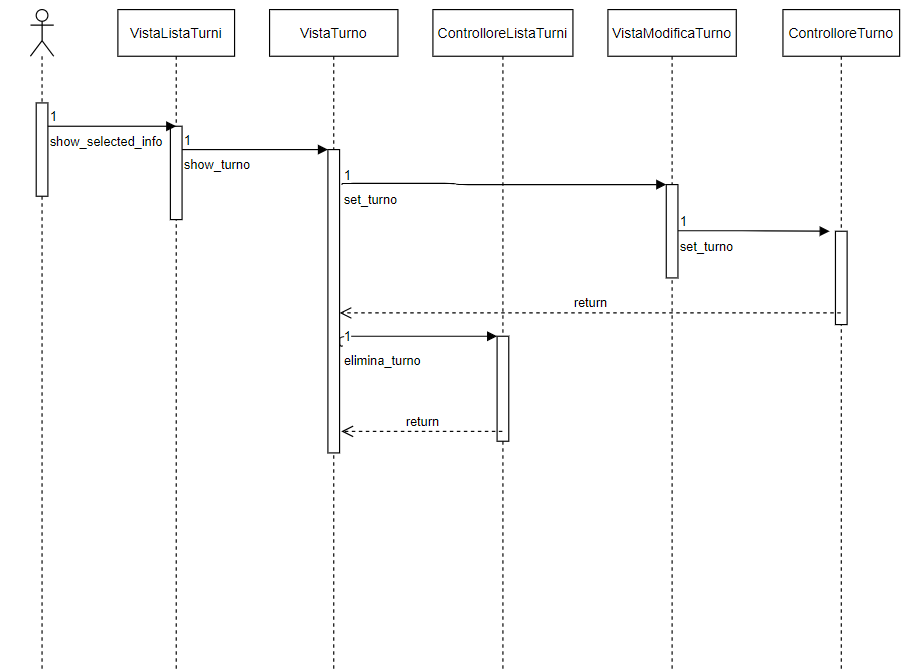
\includegraphics[scale=0.75]{sequenza_eliminaturno}
	\caption{Diagrammi delle sequenze - Eliminazione turno}
\end{figure}
\newpage
\subsection{Inserimento Utente}
\begin{figure}[H]
	\centering
	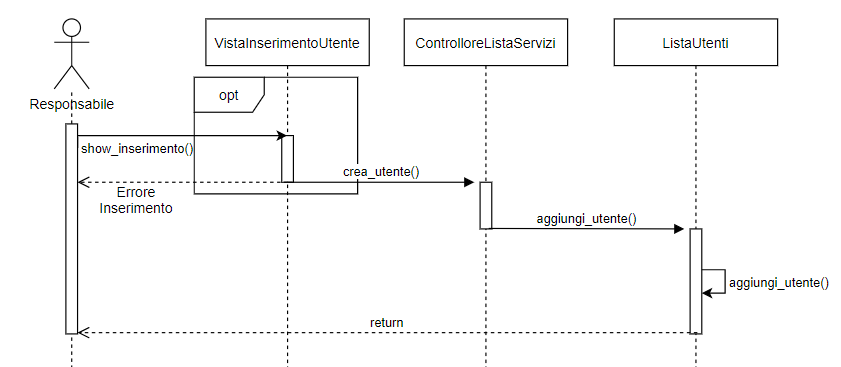
\includegraphics[scale=0.85]{sequenza_inserimentoutente}
	\caption{Diagrammi delle sequenze - Inserimento utente}
\end{figure}
\subsection{Creazione Report}
\begin{figure}[H]
	\centering
	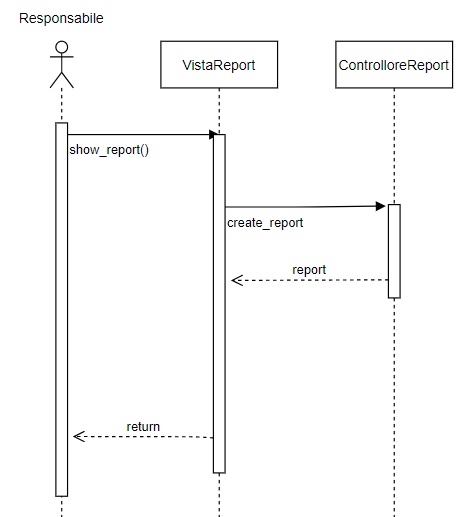
\includegraphics[scale=0.8]{sequenza_creazionereport}
	\caption{Diagrammi delle sequenze - Creazione report}
\end{figure}
\newpage
\subsection{Modifica Servizio}
\begin{figure}[H]
	\centering
	\includegraphics[scale=0.5]{Sequenza_modifica}
	\caption{Diagrammi delle sequenze - Modifica servizio}
\end{figure}
\newpage

\section{Diagrammi delle attività}
  I seguenti diagrammi delle attività sono solo una parte dei diagrammi, poiché molte delle attività prevedono una sequenza di azioni molto simili tra loro.
{\center
\subsection{Inserimento Operatore}
\begin{figure}[H]
	\centering
	\includegraphics[scale=0.75]{attività_inserimentooperatore}
	\caption{Diagrammi delle attività - Inserimento operatore}
\end{figure}
\newpage
\subsection{Modifica Operatore}
\begin{figure}[H]
	\centering
	\includegraphics[scale=0.75]{attività_modificaoperatore}
	\caption{Diagrammi delle attività - Modifica operatore}
\end{figure}
\newpage
\subsection{Creazione Report}
\begin{figure}[H]
	\centering
	\includegraphics[scale=0.75]{attività_report}
	\caption{Diagrammi delle attività - Creazione report}
\end{figure}
\newpage
}

\section{Schema Database}
Viene riportato lo schema ER del DataBase, dove vengono mostrate le entità che comporrano il DB e i loro attribuiti.
\begin{figure}[H]
	\centering
	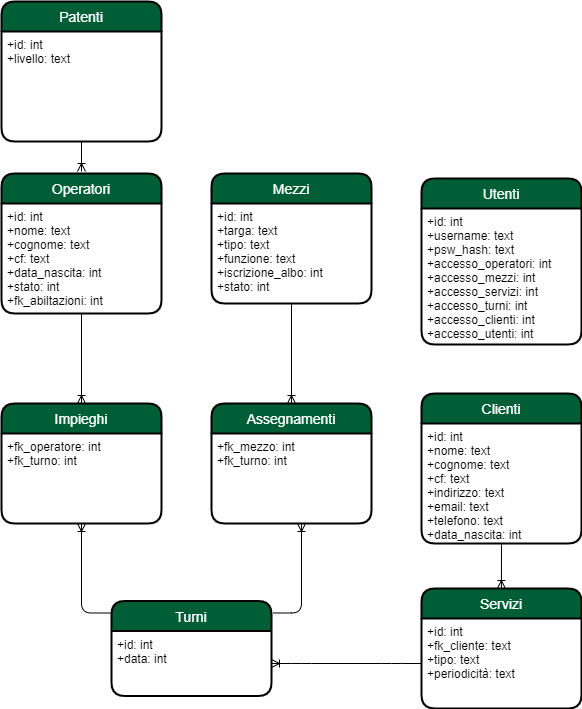
\includegraphics[scale=0.75]{schema_db4}
	\caption{Schema ER database}
\end{figure}

\newpage
\section{WireFrame}
Per l'ideazione della parte grafica del programma, in prima fase si sono progettati i WireFrame che saranno la base di partenza per l'implementazione dell'interfaccia grafica.
\begin{figure}[H]
	\centering
	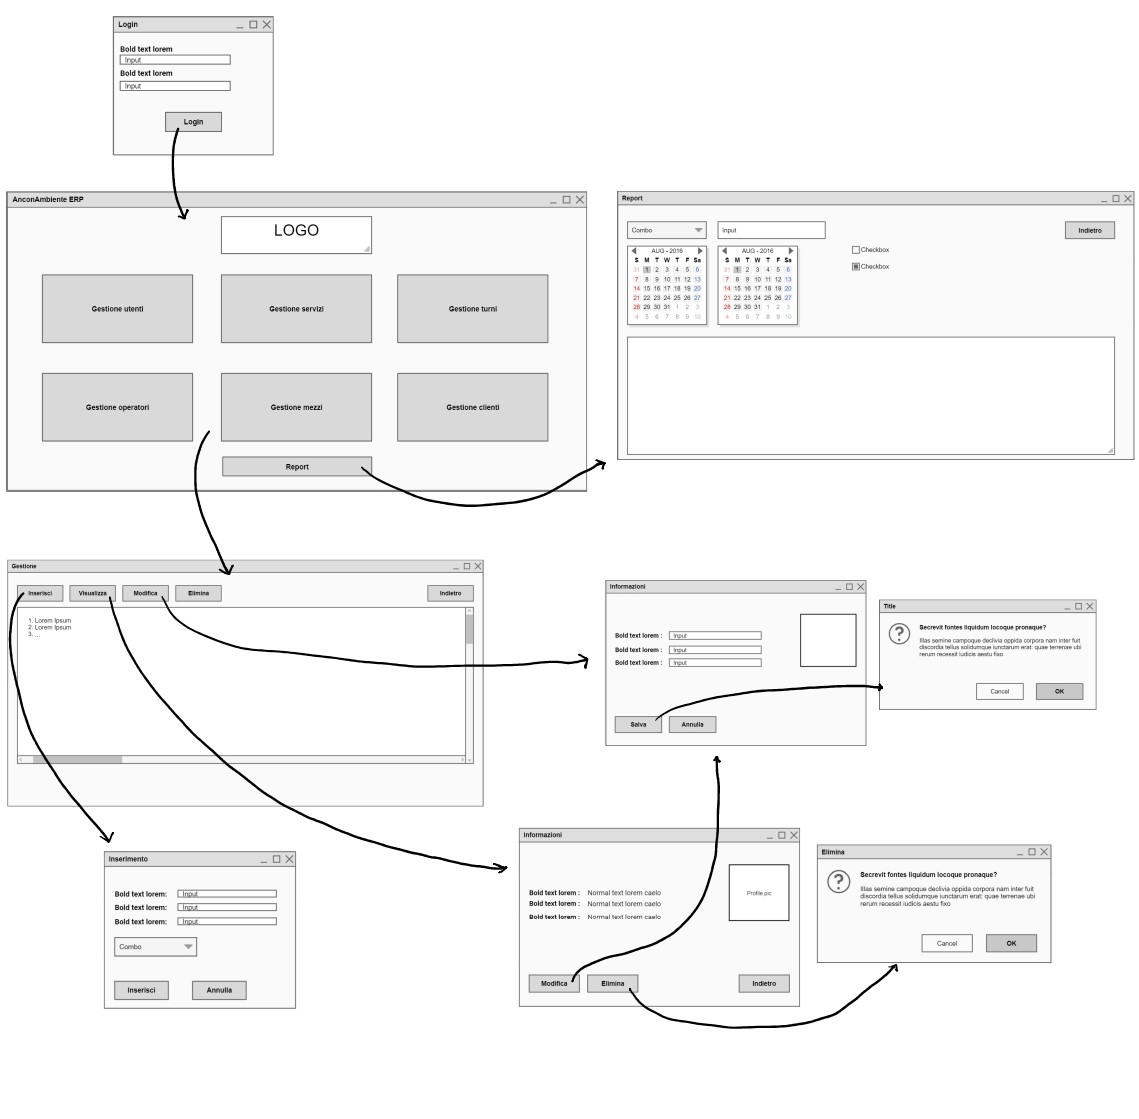
\includegraphics[scale=0.95]{wireframe}
	\caption{Wireframe}
\end{figure}

\newpage
\section{Mockup}
Partendo dalla base dei WireFrame si sono sviluppati i Mockup per pensare l'obiettivo che si vuole raggiungere al momento della implementazione della interfaccia grafica.
\begin{figure}[H]
	\centering
	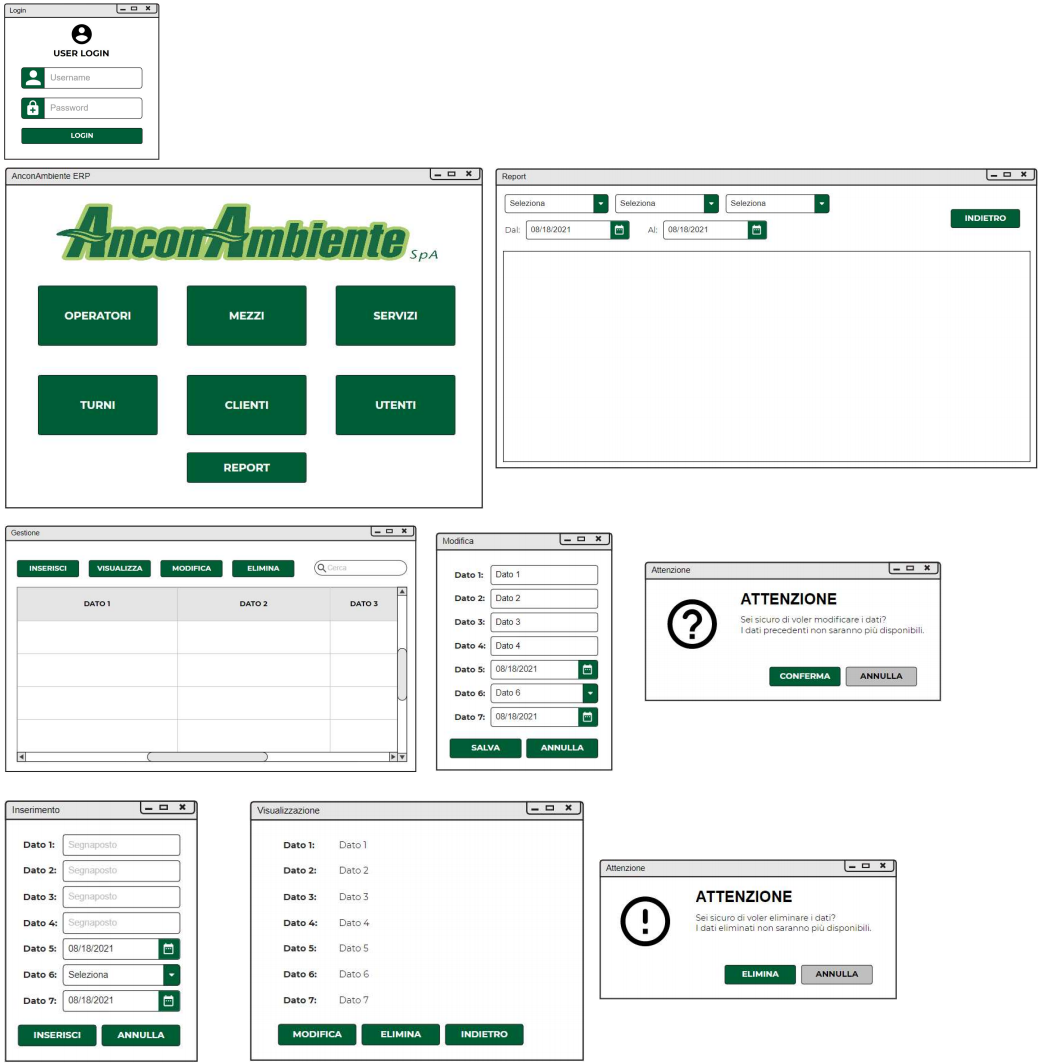
\includegraphics[scale=0.68]{mockup}
	\caption{Mockup}
\end{figure}

\newpage
\chapter{Unit Test}
Come ultima fase di progettazione, si è andato ad implementare una parte di test del Software mediante l'utilizzo del framework di automazione dei test PyUnit. 
La fase di Test è necessaria per andare a valutare se il software esegue correttamente tutti i sui compiti.

\section{Test Operatori}
Nella seguente sezione sono riportati i test sui metodi principali degli operatori.
Non sono stati eseguiti i test di mezzi, clienti, servizi ed utenti in quanto risultano essere equivalenti ad operatori.


\end{document}
